\documentclass[12pt,a4paper,american]{thesis}
\newcommand{\tipo}{Tese}
\newcommand{\tipoeng}{Thesis}
\newcommand{\grau}{Doutor}
\newcommand{\graueng}{Doctor}
\newcommand{\abrevi}{D.Sc.}
\usepackage{ifpdf}
\usepackage{times,epstopdf,ifpdf,latexsym,graphics,psfrag,ps4pdf,thumbpdf}
\usepackage{epstopdf}

\newif
  \ifpdf
  \ifx
    \pdfoutput \undefined \pdffalse
    \usepackage{graphicx}
  \else
      \usepackage[pdftex]{graphicx}

      \usepackage{epstopdf}
      \pdfcompresslevel=9
      \pdfoutput=1
      \pdftrue
    \fi
\newcommand{\pdfgraphics}{
\ifpdf
   \usepackage{graphicx,latexsym,pdftex,graphics}
   \pdfcompresslevel=9
   \DeclareGraphicsExtensions{.pdf,.png,.jpg,.jpeg,.mps}
\fi}

\usepackage[round]{natbib}
\usepackage{sty/identfirst}
\usepackage{sty/datetime}
\usepackage{sty/ulem}
\usepackage{sty/rotating}
\usepackage[T1]{fontenc}
\usepackage[latin1]{inputenc}
\usepackage[english]{babel}
\usepackage{ae}
\usepackage{color}
\usepackage{colortbl}
\usepackage{lscape}
\usepackage{caption}
\usepackage{footnote}
\usepackage{verbatim}
\usepackage{epsfig}
\usepackage{textcomp}
\usepackage{amssymb,amsmath,amsfonts}
\usepackage{mathtools}
\usepackage{eqparbox}
\usepackage{epstopdf}
\usepackage{amsthm}

\newtheorem{thm}{Theorem}[section]
\newtheorem{pro}[thm]{Proposition}
\newtheorem{cor}[thm]{Corollary}
\newtheorem{lem}[thm]{Lemma}
\newtheorem{defn}{Definition}[section]

\newcommand{\code}{\mathcal{C}}
\newcommand{\vetor}[1]{\boldsymbol{#1}}
\newcommand{\gf}{\mathbb{F}_2}
\newcommand{\parityCheckMatrix}{\normalfont\textsf{H}}
\newcommand{\generatorMatrix}{\normalfont\textsf{G}}
\newcommand{\quotes}[1]{``#1''}

\usepackage{lipsum}
\usepackage{xargs}
\usepackage[pdftex,dvipsnames]{xcolor}  
\usepackage[colorinlistoftodos,prependcaption,textsize=tiny]{todonotes}
\newcommandx{\unsure}[2][1=]{\todo[backgroundcolor=red!25,bordercolor=red,#1]{#2}}
\newcommandx{\basedon}[2][1=]{\todo[backgroundcolor=brown!25,bordercolor=brown,#1]{#2}}
\newcommandx{\change}[2][1=]{\todo[linecolor=blue,backgroundcolor=blue!25,bordercolor=blue,#1]{#2}}
\newcommandx{\info}[2][1=]{\todo[linecolor=OliveGreen,backgroundcolor=OliveGreen!25,bordercolor=OliveGreen,#1]{#2}}
\newcommandx{\improvement}[2][1=]{\todo[linecolor=Plum,backgroundcolor=Plum!25,bordercolor=Plum,#1]{#2}}
\newcommandx{\thiswillnotshow}[2][1=]{\todo[disable,#1]{#2}}


\logo{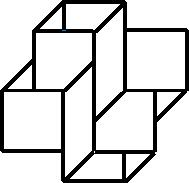
\includegraphics{logo/lncc}}
\title{Criptografia P\'os-Qu\^antica}
\titleeng{Postquantum Cryptography}
\author{Juan del Carmen}{Grados Vasquez}
\degree{\grau{} em Ciências em Modelagem Computacional }  %  #1 {long descr.}
       {\abrevi{}}                            %  #2 {short descr.}
\dept{Laborat\'orio Nacional de Computa\c c\~ao Cient\'ifica}{}
\advisor {, D.Sc}{Portugal}{Renato}
\readerTwo{, Ph.D}{Clemente Augusto Souza}{Tanajura}% 2rd Avaliador do LNCC
\readerThree{, D.Sc.}{Eduardo Lúcio Mendes}{Garcia} % 3rd Avaliador do LNCC
\readerFour {, D.Sc.}{Fulano de}{Tal}               % 4rd Avaliador de Instituicao Externa
\readerFive {, Ph.D}{Ciclano de}{Tal}               % 5rd Avaliador de Instituicao Externa

\readerSix{, Ph.D}{Beltrano de}{Tal}                % 6th Avaliador de 
\catalography[Ficha Catalogr\'afica]{\OnePageChapter
\familyname{Gazoni} \givenname{Leandro Carlos}

\numpages{xx, yy p.}
\keyword{1. HashBased Cryptography. 2. Multivariate. 3. Coding Theory. 4. palava chave. }

\codbib{CDD xxx.xxx} \codtese{XXXX} }

\abstract{  \OnePageChapter
  Aqui entra o resumo de seu trabalho em portugu�s.
}

\abstracteng{  \OnePageChapter  % one page only
  Here, you type your abstract in english
}

\inspiration[]{ \OnePageChapter % NEVER use \OnePageChapter here.
  \textbf{e.p�.gra.fe}\\
    s. f. 1. Senten�a ou divisa posta no frontisp�cio de um livro ou
    cap�tulo, no come�o de um discurso ou de uma composi��o po�tica.
    2.Inscri��o posta em lugar vis�vel de um edif�cio.\\
    \tiny{\textit{(Fonte: Dic. Aur�lio.)}}
 }

\dedication[]
{
    \OnePageChapter % NEVER use \OnePageChapter here.

    \textbf{To my wife and daugther}\\
    \textbf{for her love}
    %Men��o que o autor faz (homenagem) em folha distinta.


}

\acknowledgements{
\OnePageChapter % *MUST* BE ONLY ONE PAGE!

O autor manifesta reconhecimentos �s pessoas e institui��es que
colaboraram para a execu��o de seu trabalho.

}

\symbols{	\OnePageChapter	% *MUST* BE ONLY ONE PAGE!
{\footnotesize
\begin{itemize}
\item 1ME4: cristal da cruzipa�na 1, obtido do PDB
\item 1ME4m: modelo da cruzipa�na 2, gerado a partir do cristal 1ME4
\item 24-SMT: 24-metiltransferase
\item 3D: Tridimensional
\item 9PAP: cristal da papa�na, obtido do PDB
\item $\mathring{A}$: Angstroms
\item AK: Arginina cinase
\item ALA: Alanina
\item ARG: Arginina
\item ASN: Asparagina
\item ASP: �cido asp�rtico
\item BATS: {\it BLAST Automatic Targeting for Structures}
\item BLAST: {\it Basic Local Alignment Search Tool}
\item C$_\alpha$: Carbono-$\alpha$
\item CDS: Sequ�ncia codificante
\item Cl$^-$: �on Cloro
\item CSO: S-Hidroxiciste�na
\item CYP51: Citocromo-P450 em {\it T. cruzi}
\item CYS: Ciste�na
\item DM: Din�mica Molecular
\item DNA (ou ADN): �cido Desoxirribonucl�ico
\item EC: Classifica��o Enzim�tica
\item ED$_{50}$: Dose M�dia Efetiva
\item FTase: Farnesiltransferase
\item GLN: Glutamina
\item GLU: �cido glut�mico
\item gp = GP: Glicoprote�na
\item GPI: Glicosilfosfatidilinositol
\item GR: glutationa redutase
\item GRSI: {\it Gap Relative Strengh Index}
\item {\it H. sapiens} = {\it h} =  HSA: {\it Homo sapiens}
\item HIS: Histidina
\item IC$_{50}$: Concentra��o M�dia Inibit�ria
\item ID$_{50}$: Dose M�dia Inibit�ria
\item K$_i$: Constante de dissocia��o
\item KEGG: {\it Kyoto Encyclopedia of Genes and Genomes}
\item LC$_{50}$: Concentra��o M�dia Letal
\item LEU: Leucina
\item LIT: {\it Liver Infusion Tryptose}
\item LVI: {\it Lenght Variation Index}
\item LYS: Lisina
\item MET: Metionina
\item MIC: Concentra��o M�nima Inibit�ria
\item Na$^+$: �on S�dio
\item NADH: estado reduzido da Nicotinamida Adenina Dinucleot�deo (NAD)
\item NC-IUBMB: {\it Nomenclature Committee
	 of the International Union of Biochemistry and Molecular
	 Biology} 
\item PDB: {\it Protein Data Bank}
\item PDF: Fun��o Densidade de Probabilidade
\item PHE: Fenilalanina
\item PRO: Prolina
\item RMN: Resson�ncia Magn�tica Nuclear
\item RMSD: Desvio M�dio Quadr�tico
\item Rx: Raios-X
\item SAS: Superf�cie Acess�vel ao Solvente
\item SER: Serina
\item SQS: Esqualeno sintase
\item S-S: Liga��o dissulf�dica
\item {\it T. cruzi} = {\it Tc} = TCR: {\it Trypanosoma cruzi}
\item TR: Tripanotiona redutase
\item TRP: Triptofano
\item TYR: Tirosina
\item TS: Trans-sialidase
\item T[SH]$_2$: Tripanotiona (N$^1$,N$^8$-bis(glutationil)spermidina) redutase
\item UNG: Uracil-DNA glicosilase
\item VAL: Valina
\end{itemize}
}
}


%Insert Table of Contents (chapter, bibliography and apendix)
\ToCisShort % a 1-page Table of Contents

%Insert (or not) List of figures
\LoFisShort % a 1-page List of Figures
%\emptyLoF  % no List of Figures at all
\LoTisShort % a 1-page List of Tables
\begin{document}
\selectlanguage{english}

\chapter{{Introduction}}
\section{Contribution of this thesis}


\pagestyle{empty}
\todo[inline]{The original todo note withouth changed colours.\newline Here's another line.}
\lipsum[11]\unsure{Is this correct?}\unsure{I'm unsure about also!}
\lipsum[11]\change{Change this!}
\lipsum[11]\info{This can help me in chapter seven!}
\lipsum[11]\improvement{This really needs to be improved!\newline\newline What was I thinking?!}
\lipsum[11]
\thiswillnotshow{This is hidden since option `disable' is chosen!}
\improvement[inline]{The following section needs to be rewritten!}
\lipsum[11]
\newpage
\listoftodos[Notes]

\part{Background}
%\include{chapters/chapter_background_finite_field}
\chapter{{Hash Based Cryptography}}

%!tex root = ../thesis.tex
\chapter{{Coding Based Cryptography}}
In 1948 Shannon published one of his most celebrated works \quotes{A Mathematical Theory of Communication}. Here were established the bases of the coding theory and the information theory. The coding theory was initially created with the object of studying how to encode messages on a noisy channel communication. Over the years this theory has growing, and now it includes the study of codes, including error detecting codes and error correcting codes. 

There are several areas where the coding theory is applied, for example in data compression, cryptography, error-correction, and networking. The following is a classic example in the error-correction area. In 1971 was launched Mariner 71, a spacecraft which, among other missions, should to send pictures from Mars to the Earth. To transmit these pictures a fine grid was placed over the picture. In each square was quantified the blackness degree of the picture with a number between $0$ and $63$. These numbers were represented with a binary string of length $6$. The bits $0$ and $1$ were transmitted as two different signals to a receiver station in the Earth. However, sometimes the signals arrived weak due to great distance. This caused sometimes $0$ was understood as $1$, and vice versa. Though, Mariner was equipped with the Reed Salomon code. As other codes, this  code  incorporates some redundancy, so that, if some of the symbols in a codeword are changed, we can still figure out the transmitted message. In the case of Reed Salomon used for Mariner 71 the codeword consists of $m$ bits of original data and $n$ bits of redundancy. That instance of the code is called $(6,4)$ Reed Salomon code and in section we are going to explain that in more detail.

In 1978 that theory was also used by McEliece to create a public key cryptosystem and the code used at this time was the Goppa codes. Since that time many new cryptosystems using code theory have appeared. These cryptosystems initially did not call much attention because the size of its keys, but with the imminent arrival of the quantum computers these cryptosystems came afloat because they resist attacks that use this type of computers. To understand these cryptosystems first is necessary to know some mathematical background about codes and .... In this chapter we will give an overview of the main definitions and theorems that we will need in the thesis, for more information please refer to A and B.

\section{Linear Codes}

Linear codes are the cornerstone for almost all code based cryptosystems. Traditionally the linear codes are partitioned in two: the block codes and the convutional codes. The cryptosystems we are going to present in this chapter uses block codes. In this kind of codes the message to be transmitted are divided in blocks of equal size and each one of these blocks can be code and decoded independently. These blocks are called \textit{codewords} and the size $n$ of one block is just called of \textit{lenght} of the code. The messages are coded on a alphabet. In this thesis we are use the $\mathbb{F}_2$ finite field as alphabet unless we mention otherwise.

{
    \defn{[33, \cite{Lint:1998:ICT:552386}]} If $\vetor{x}\in \mathbb{F}_2^n$, $\vetor{y}\in \mathbb{F}_2^n$, then the distance $d(\vetor{x},\vetor{y})$ of $\vetor{x}$ and $\vetor{y}$ is defined by
    
    \[
        d(\vetor{x},\vetor{y}) \coloneqq |\left\{i|1\leq i \leq n, x_i \neq y_i\right\}|
        \]
    
    The weight $w(\vetor{x})$ of $\vetor{x}$ is defined by 
    
    \[
        w(\vetor{x})\coloneqq d(\vetor{x},\vetor{0}).
    \]
}

(We always denote $(0,0,\cdots,0)$ by $\vetor{0}$ and $(1,1,\cdots,1)$ by  $\vetor{1}$.)

The distance defined above is called \textit{Hamming-distance}. 
In the following a code $\mathcal{C}$ is a nonempty proper subset of $\mathbb{F}_2^n$. The following concepts play an essential role in this thesis

{
    \defn{[34, \cite{Lint:1998:ICT:552386}]} The minimum distance of a code $\code$ is 
    \[
        \min\left\{d(\vetor{x}, \vetor{y})|\vetor{x}\in \code, \vetor{y} \in \code, \vetor{x}\neq \vetor{y}\right\}.
    \]
    
    For a linear code the minimum distance is the minimal weight of a non-zero codeword. In other words the minimum distance of a linear $\code$ is
    
    \[
        \min\left\{ w(\vetor{x}) |  \vetor{x} \in \code, \vetor{x}\neq \vetor{0}\right\}.
    \]
}
{
    \defn{[34, \cite{Lint:1998:ICT:552386}]} 
    \[
        R\coloneqq n^{-1}\log_2|\code|
    \]
    is called the rate of $\code$
}

In coding theory, a linear code is an error-correcting code for which any linear combination of codewords is also a codeword. More formally.

{
    \defn{[35, \cite{Lint:1998:ICT:552386}]} A q-ary linear code $\code$ is a linear subspace of $\gf^n$. If $\code$ has dimension $k$ then $\code$ is called an $[n,k]$ code.
}

Hereafter, we shall use $[n,k,d]$ code as the notation for a $k$-dimensional linear code of length $n$ and minimum distance $d$.

{
    \defn{[35, \cite{Lint:1998:ICT:552386}]} A generator matrix $\generatorMatrix$ for a linear code $\code$ is a $k$ by $n$ matrix for which the rows are a basis of $\code$.
}

A code $\code$ can be described by its generator matrix, in other words if $\generatorMatrix$ is a generator matrix for $\code$, then $\code = \left\{\vetor{a}\generatorMatrix|\vetor{a}\in \gf^k\right\}$. We shall say that $\generatorMatrix$ is in standard form (or reduced echelon form) if $\generatorMatrix = (I_k\,\,P)$, where $I_k$ is the identity matrix with dimensions $k\times k$. If $\generatorMatrix$ is in standard form then the first $k$ symbols are called of information symbols and the remaining of parity check symbols.

{
    \defn{[4, \cite{Lint:1998:ICT:552386}]} Given $\vetor{a}\coloneqq (a_1, a_2, \cdots, a_n)$ and $\vetor{b}\coloneqq (b_1, b_2, \cdots, b_n)$. The inner product $\langle\vetor{x},\vetor{y}\rangle$ is defined by
    \[
        \langle\vetor{x},\vetor{y}\rangle \coloneqq a_1b_1 + a_2b_2 + \cdots + a_nb_n.
    \]
}

{
    \defn{[36, \cite{Lint:1998:ICT:552386}]} If $\code$ is a $[n,k]$ code we define the dual code $\code^{\perp}$ by 
    \[
        \code^{\perp} \coloneqq \left\{\vetor{y}\in \gf^n | \forall _{\vetor{x}\in \code}\left[\langle\vetor{x},\vetor{y}\rangle = 0\right]\right\}.
    \]
}

The dual code $\code^{\perp}$ is clearly a linear code, namely $\left[n,n-k\right]$ code. If $\generatorMatrix=(I_k\,\,P)$ is a generator matrix in standard form of the code $\code$, then $\parityCheckMatrix = (-P^{T}\,\,I_{n-k})$ is a generator matrix for $\code^{\perp}$. This follows from the fact that $\parityCheckMatrix$ has the right size and rank and that $G\parityCheckMatrix^T = 0$ implies that every codeword $\vetor{a}G$ has inner product $0$ with every row of $\parityCheckMatrix$. More formally
\[
    \vetor{x} \in \code \iff \vetor{x}\parityCheckMatrix^T = \vetor{0}.
\]
$\parityCheckMatrix$ is called of parity check matrix of $\code$


{
    \defn{[36, \cite{Lint:1998:ICT:552386}]} If $\code$ is a linear code with parity check matrix $\parityCheckMatrix$ then for every $\vetor{x}\in\gf^n$ we call $\vetor{x}\parityCheckMatrix^T$ of the syndrome of $\vetor{x}$. 
}


{
\thm{[67, \cite{Richard}]}
    Let $\code$ be a linear code with parity matrix $\parityCheckMatrix$ and $s$ the minimum number of linearly dependent columns in $ \parityCheckMatrix $, then $s$ is the minimum distance of the code.
}

\textit{Proof}. Let $d$ be the minimum distance of $\code$ and let $\vetor{x}= (x_1, \cdots x_s, 0, \cdots, 0)$ $\in \code$ where $x_i \neq 0 $ in the range $1 \leq i \leq s$. Obviously, $s$ can not be less than $d$, because in that case $s$ must be the minimum distance of the code. It remains to prove that $s$ can not be greater than $d$. Let $\vetor{y} = (y_1, \cdots y_d, 0,0, \cdots, 0) \in C$, with $y_i \neq 0$ in range $ 1 \leq i \leq d$. Since $\vetor{y} \in \code$ then $\parityCheckMatrix\vetor{y}=0$, that is, we have found $d$ linearly dependent columns. Now $s$ can not greater than $d$ because this violates the hypothesis: $s$ is the minimum number of linearly dependent columns in $ \parityCheckMatrix$.

\section{Decoding Problems}
In some code based cryptosystems the next theorem is important because helps to guarantee the hardness of cryptosystems against certain types of attacks.
{
\thm{[3, \cite{Barreto:2011:OSS:1922690.1922979}]}
    A binary linear code $[n,k,d]-\code$ is ensured to exist as long as:
\[
  \sum_{j=0}^{d-2}\binom{n-1}{j}<2^{n-k}.
\]
}
This is called the Gilbert-Varshamov (GV) bound. Random binary codes are known to meet the GV bound, in the sense that the above inequality comes very close to being an equality \cite{book:MacWilliams:Sloane}. No family of binary codes is known that can be decoded in subexponential time up to the GV bound, nor is any subexponential algorithm known that can decode general codes
up to the GV bound. In follow we present the proof of this theorem following as reference \cite{book:MacWilliams:Sloane}.




%From then until now several 
%representing words of a code as its rank in some conventional ordering

\chapter{{SAT Problem}}
\label{chap:satisfiability}

In our thesis we studied the security of multivariate cryptography from the perspective of solving instances of the Boolean Satisfiability Problem, which is also known as the SAT problem. 

%Thus, before this study we focused on the concepts of the SAT problem starting by defining itself. After, we will describe a special case of the SAT problem which is widely used in multivariate cryptography.

The SAT problem is defined as follows. First, one is given a logical expression in the five operators of predicate calculus $(\wedge, \vee, \neg, \Rightarrow, \iff )$ but not the existential or universal quantifiers ($\exists, \forall$). Then, one is asked if the logical expression has a assignment for each of its variables, such that the logical expression evaluates to true. Unlike, the problem if the expression has the value false, for every one its possible assignments, is called UNSAT.\basedon{\cite[p. 200]{bard2009algebraic}}

The solving of the SAT problem has been extensively studied along of years and many methods to solve it have been developed. The most efficient methods seem to be all derived from the method proposed by \cite{davis1958reductions}. Their proposal uses as input a logical expression in Conjunctive Normal Norm (CNF). A formula is in CNF form if it is a conjunction of clauses, and each clause is a disjunction of literals. 

In follow, we define these concepts more formally.

\begin{defn}
The language of Boolean formulae consists of Boolean variables, whose values are True or False; Boolean operators such as negation $(not)$, conjunction $(\wedge)$, disjunction $(\vee)$, implication $(\Rightarrow)$, equivalence $(\iff)$; and parentheses.
\end{defn}

\begin{defn}
A literal is either an atomic formula or the negation of an atomic formula.
\end{defn}

\begin{defn}
A clause is a disjunction of $n >0$ literals
\end{defn}
The most study and promises SAT solvers are based on the work of Davis and Putnam. In this thesis, for the cryptanalysis against multivariate quadratic scheme we use a kind of solvers called Clause Driven Clause Learn SAT (CDCL-SAT). As we will see, these SAT solver are inspired on the Davis and Putnam method and uses as input a logical expression in CNF. 

%https://www8.cs.umu.se/kurser/TDBAfl/VT06/algorithms/BOOK/BOOK3/NODE112.HTM
When the maximum number of literals presented in each clause of a CNF logical expression is $k$, then the respective SAT problem is known as $k$-CNF-SAT problem. Since clause sets with only one literal per clause are easy to satisfy, the computer scientist, and particularly in this thesis, we are interested in slightly larger classes. Exactly what is the clause size at which the problem turns from polynomial to hard? This transition occurs when each clause contains three literals, the so-called $3$-CNF-SAT problem. Follow there is a formalization of the $3$-CNF-SAT problem.\\
\\
\noindent
\textbf{3-CNF-SAT Problem.} Let $B=\{b_1,\cdots,b_n\}$ be a set of Boolean variables, let $L=\left\{b_1,\overline{b_1},\cdots,b_n,\overline{b_n}\right\}$ be the corresponding set of literals, let $c_i\in \left(L\cup L^2\cup L^3\right)$ be clauses of at most 3 literals, and let $C=\left\{ c_1, \cdots, c_m\right\}$ be a set of these clauses. Then the corresponding 3-CNF-SAT problem is to determine if there is an assignment $A\in \left\{0,1\right\}^n$ for $B$ such that all $c_i$ are true and hence $C$ is satisfied.\\
\\
\noindent
The worse-case estimates for solving SAT on a CNF problem are commonly given in terms of the numbers of clauses $c$, number of variables $v$, the total length of all clauses $L$, and the Strahler number of the tree-like resolution proof. In section we will review several methods for trying to formalize the hardness of solving SAT problems.
%Thus, logical expression encoding as 3-CNF-SAT problems are most efficient to solve when the number of variables $n$ is used a measure of difficulty of the $k$-CNF-SAT problems. Thus, in this thesis we encoding our multivariate quadratic systems as 3-CNF-SAT problems.



%\textbf{SAT-Problem.} Give a Boolean formula $\Phi$ of $n$ variables and $m$ clauses. Is there any model for $\Phi$?\\
%\\
%\noindent

\chapter{{Multivariate Cryptography}}

%falar de multivariados em general
\section{Basic Notation}
%Falta corregir hablar de multivariables en general
In the context of multivariate cryptography, we mostly deal with systems of multivariate quadratic polynomials functions over finite fields. In this work, by $\mathbb{F}_q$, or GF($q$) we denote a finite field consisting of $q$ elements, and by $\mathbb{E}$ a extension field of $\mathbb{F}_q$. By $\mathbb{F}_q^n$ we shall denote the vector space of $n$-tuples over $\mathbb{F}_q$. Elements of $\mathbb{F}_q^n$ are denoted by bold characters.

A multivariate quadratic system of polynomials functions with $n$ variables and $m$ equations has the following form
\begin{equation}
p^{(k)}(x_1,x_2,\cdots,x_n) = \sum_{1\leq i \leq j \leq n}\gamma_{i,j}^{(k)} x_i x_j + \sum_{i=1}^{n}\beta^{(k)}_i x_i + \alpha^{(k)}
\label{eq:1}
\end{equation}
where $1\leq k\leq m$ and $\gamma_{i,j}^{(k)}, \beta^{(k)}, \alpha^{(k)} \in \mathbb{F}_q$. If $m=n$ the system is called determined, if $m>n$ the system is called overdetermined and if $m<n$ the system is called undetermined. We call $\gamma_{i,j}^{(k)}, \beta^{(k)}, \alpha^{(k)}$ coefficients and $x_ix_j, x_i$ monomials. The product of a coefficient with  a monomial is called a term. We call a multivariate quadratic system $P$ homogeneous if it not contains linear, nor constants terms.
%Setting $y^{(k)} = p^{(k)}(x_1,x_2,\cdots,x_n) = \sum_{1\leq i \leq j \leq n}\gamma_{i,j}^{(k)} x_i x_j + \sum_{i=1}^{n}\beta^{(k)}_i x_i + \alpha^{(k)}$ we, can express \ref{eq:1} as a set of polynomial functions.

A multivariate quadratic system can be expressed as a set 
\[
P:=\{p^{(1)}, p^{(2)}, p^{(3)}\cdots p^{(m)}\}
\] 
of polynomial functions or in equivalent way as a quadratic map $P\colon \mathbb{F}_q^n \rightarrow \mathbb{F}_q^m$

\begin{equation}
 P=\left(\begin{matrix}
    p^{(1)}(x_1,x_2,\cdots,x_n)  \\
    p^{(2)}(x_1,x_2,\cdots,x_n) \\
    \vdots \\
    p^{(m)} (x_1,x_2,\cdots,x_n) 
   \end{matrix}\right).
\label{eq:maprepresentation}
\end{equation}
\noindent
\textbf{Matrix Representation}.
It is possible to write each polynomial function of \eqref{eq:maprepresentation} $p^{(k)}$ as a matrix-vector product using the upper triangular matrix 

\begin{equation}
 P^{(k)}=\left[\begin{matrix}
   \gamma_{1,1}^{(k)} & \gamma_{1,2}^{(k)} & \gamma_{1,3}^{(k)} & \cdots & \gamma_{1,n}^{(k)} & \beta_{1}^{(k)}\\
  0 & \gamma_{2,2}^{(k)} & \gamma_{2,3}^{(k)} & \cdots & \gamma_{2,n}^{(k)} & \beta_{2}^{(k)}\\
  0 & 0 & \gamma_{3,3}^{(k)} & \cdots & \gamma_{3,n}^{(k)} & \beta_{3}^{(k)}\\
  \vdots &  & \ddots &  & \vdots & \vdots\\  
  0 & 0 & \cdots & 0 & \gamma_{n,n}^{(k)} & \beta_{n}^{(k)}\\
   0 & 0 & \cdots & 0 & 0 & \alpha^{k} 
   \end{matrix}\right]
\label{eq:3}
\end{equation}
and the vector $(x_1,x_2,x_3,\cdots,x_n,1)$ in the following form
\begin{equation}
p^{(k)} = (x_1,x_2,x_3,\cdots,x_n,1) P^{(k)} (x_1,x_2,x_3,\cdots,x_n,1)^{T}
\end{equation}

Although, this construction seems strange this will be useful at the chapter \ref{chapter:mpqc} when, we talked about Attacks on Multivariate Quadratic Schemes.

\section{The Standard (Bipolar) Construction}
The standard and most popular construction of multivariate cryptography consists of select a map $P\colon\mathbb{F}_q^{n}\rightarrow \mathbb{F}_q^{m}$ of polynomials functions of degree two as \eqref{eq:maprepresentation}, such that it is easy to find pre-images. Besides, chooses two affine transformations $S\colon\mathbb{F}_q^{m}\rightarrow \mathbb{F}_q^{m}$ and $T\colon\mathbb{F}_q^{n}\rightarrow \mathbb{F}_q^{n}$. These objects are used to construct encryption and signature schemes and we will see that for encryption is necessary that $m\geq n$ and for signature is necessary that $m\leq n$. The public key is the composition $\bar{P} = S \circ P \circ T$ and the private key consists of $S$, $P$ and $T$.\\
\noindent
\textbf{Encryption Schemes}\\
\noindent
\textit{Encryption.} To encrypt a message $\boldsymbol{m}$, it is only necessary compute $\boldsymbol{c} = \bar{P}(\boldsymbol{m})$. The ciphertext of the message $\boldsymbol{m}$ is $\boldsymbol{c}$.\\
\noindent
\textit{Decryption.} To decrypt the ciphertext $\boldsymbol{c}$ is necessary compute $\boldsymbol{y} = S^{-1}(\boldsymbol{c})$, $\boldsymbol{y'} = \bar{P}^{-1}(\boldsymbol{y})$ and the original message is $\boldsymbol{m} = T^{-1}(\boldsymbol{y'})$. Note that $P^{-1}$ do not denote the inverse functions, which might not even exist, but some pre-image. In other words, sometimes is possible to exist another pre-images $\boldsymbol{m_1}, \boldsymbol{m_2}, \cdots \boldsymbol{m_k}$ such that $\bar{P}(\boldsymbol{m_1}) = \bar{P}(\boldsymbol{m_2}) = \cdots = \bar{P}(\boldsymbol{m_k}) = \bar{P}(\boldsymbol{m})$. This problem has been discussed by \cite{Patarin1996} and he suggest to use error correcting codes or hash function to solve it. 

We say that for encryption is necessary that $m\geq n$ because in this case with high probability there is a unique pre-image of $\boldsymbol{y}$ under $\bar{P}$.\\
\noindent
\textbf{Signature Schemes}\\
\noindent
\textit{Signature Generation.} To sign a document $d$, we calculate $\boldsymbol{h} = H(d)$ where $H$ is a hash function. Then we compute $\boldsymbol{y} = S^{-1}(\boldsymbol{h})$, $\boldsymbol{y'} = \bar{P}^{-1}(\boldsymbol{y})$ and the signature of $\boldsymbol{h}$ is $\boldsymbol{z} = T^{-1}(\boldsymbol{y'})$. Again, note that $P^{-1}$ do not denote the inverse functions, which might not even exist, but any pre-image. 

We say that for signature $n \geq m$ because thus we can be sure that such a pre-image exists.
Thus, every message has a signature.\\
\noindent
\textit{Signature Verification.} To verify the  signature $\boldsymbol{z}$ of the document $d$, we compute $P(\boldsymbol{z})$ if the result equal to $\boldsymbol{h}$ the signature is accepted, otherwise it is rejected.\\
\noindent\\
\noindent
\cite{Schneier1995} argued that the use of  hash functions in cryptography schemes 
is that in practical implementations, public-key algorithms are often too inefficient to sign long documents. Thus, to save time, digital signature protocols are often implemented with hash functions. Also, hash functions are used to decrease any pattern or any known structure of a message to sign. 

The security of bipolar constructions is based on the MQ-Problem and IP-Problem problems. The MQ-Problem is proved NP-Complete but not the IP-problem, this fact difficult to construct provable security schemes based on multivariate quadratic systems.
\subsection{Example}
We shall give an example of a standard construction namely Random Singular Simultaneous Equation (R(S)SE) which was proposed by \citet{KasaharaS04}. The reason to chose this is that its simplicity for construction.\\\\
%that is a variation of the scheme  STS proposed by \cite{Tsujii1985}
\noindent
\textit{Key Generation.} The map $P$ in R(S)SE has $L$ layers of polynomials functions. Let $i$ be a $i^{th}$ layer. Each layer has $r_i$ new variables and $m_i$ equations. The $r_i$ values are such that $\sum_{i=1}^{L}r_i=n$ and the $m_i$ values are such that $\sum_{i=1}^{L}r_i=m$. In Figure \ref{fig:RSSE}, we depict the form of the map $P$ for the R(S)SE scheme. 

The public key $\bar{P}$ is constructed by using two affine transformations  $S\colon\mathbb{F}_q^{m}\rightarrow \mathbb{F}_q^{m}$ and $T\colon\mathbb{F}_q^{n}\rightarrow \mathbb{F}_q^{n}$. These two transformations are operated with $\bar{P}$ in the following way $\bar{P} = S \circ P \circ T$. The private key consists of $S$, $P$ and $T$.\\
\noindent
\textit{Encryption.} To encrypt a message $\boldsymbol m$ we only has to evaluate this message in the map $\bar{P}$, i.e. the ciphertext $\boldsymbol c = \bar{P}(\boldsymbol m)$.\\
\noindent
\textit{Decryption.} To decrypt the ciphertext $\boldsymbol c$, we first apply the inverse of the affine transformation $T$ in $\boldsymbol c$. i.e. $\boldsymbol y = T^{-1}(\boldsymbol c)$. After that, we must, to find the pre-image $\boldsymbol x$ of the system $\boldsymbol y = P(\boldsymbol x)$. To calculate the pre-image we need to construct $L$ sub-systems. The left side of each sub-systems has the form as each layer of Figure \ref{fig:RSSE}. To calculate the right side of each sub-system we need to split $\boldsymbol y$ in $L$ layers $\boldsymbol y_1, \boldsymbol y_1, \cdots \boldsymbol y_L$. Each layer $\boldsymbol y_1, \boldsymbol y_1, \cdots \boldsymbol y_L$ has $m_1, m_2, \cdots, m_L$ elements respectively. For the Layer 1, we must compute an vector of variables $\boldsymbol x_1$ for the given vector $\boldsymbol y_1$ such that $\boldsymbol x_1$ has $r_1$ entries. To compute $\boldsymbol x_1$, we need to use brute force, that is, to  compute $\boldsymbol x_1$ it is necessary to make $q^{r_1}$ attempts. After one, we compute a vector of variables $\boldsymbol x_2$ for the given vector $\boldsymbol y_2$ such that $\boldsymbol x_2$ has $r_2$ entries. Again, to compute $\boldsymbol x_2$ we must, to use brute force, that is, to compute $\boldsymbol x_2$ it is necessary to make $q^{r_2}$ attempts. These steps are repeated until we calculate the last vector of variables $\boldsymbol x_L$ with $r_L$ variables. Note, that following the construction of R(S)SE, we are finding $r_i$ new variables in each step. Putting all $\boldsymbol x_i$ together in $x$ we retrieve the original message setting $\boldsymbol m = S^{-1}(\boldsymbol x)$. Note, that in order to obtain a practical scheme the value of $r$ must be small, otherwise a legitimate user has a workload to decrypt.

\begin{figure}
\footnotesize
\[
 P=\left(\begin{array}{l}
 \text{Layer 1}  \left\{\begin{array}{l}
    p^{(1)}(x_1,x_2,\cdots,x_{r_1})  \\
    \quad\quad\vdots\\
    p^{(m_1)}(x_1,x_2,\cdots,x_{r_1})
    \end{array}
    \right.%%%%%%%%%%%%%
    \\
 \text{Layer 2}   \left\{\begin{array}{l}
    p^{(m_1+1)}(x_1,x_2,\cdots,x_{r_1}, x_{r_1+1},x_{r_1+2},\cdots,x_{r_2})  \\
    \quad\quad\vdots\\
    p^{(m_1+m_2)}(x_1,x_2,\cdots,x_{r_1}, x_{r_1+1},x_{r_1+2},\cdots,x_{r_2}) 
     \end{array}
    \right.%%%%%%%%%%%%
   \\
   \quad\quad\quad\quad\quad \quad\quad\quad\quad\quad \vdots\\
 \text{Layer L}   \left\{\begin{array}{l}
   p^{\left(m_{L-1}+1\right)}(x_1,\cdots,x_{r_1}, x_{r_1+1},\cdots,x_{r_2},\cdots, x_{n_{L-1}+1}, \cdots, x_{n_{L-1}+n_L})  \\
    \quad\quad\vdots\\
    p^{(m_{L-1}+m_L)}(x_1,\cdots,x_{r_1}, x_{r_1+1},\cdots,x_{r_2},\cdots, x_{n_{L-1}+1}, \cdots, x_{n_{L-1}+n_L}) \\
   \end{array}\right.
   \end{array}
   \right)
\]
\caption{map $P$ of (R(S)SE)}
\label{fig:RSSE}
\end{figure}
\section{The MQ Problem}
 
As we said, the security of multivariate quadratic schemes relies on the computational hardness of solving large multivariate systems. This problem, called here, the MQ-problem is enunciated as follow. \\
\\
\noindent
\textbf{MQ-Problem.} Given a system $P=\left(p^{(1)}),\cdots, p^{(m)}\right)$ of $m$ non-linear polynomials functions in the variables $x_1,\cdots, x_n$. Is there some $\overline{x_1}, \cdots, \overline{x_n}$ such that $p^{(1)}(x_1,\cdots, x_n)=0, \cdots, p^{(m)}(x_1,\cdots, x_n) = 0$?\\
\\
\noindent
Even for the case of non-linear polynomial functions of degree 2, this problem is proved NP-complete. To show that, it is necessary to reduce the 3-CNF-SAT Problem to the MQ-Problem. A proof of this reduction can be found in the thesis of \cite{wolfphdthesis}. 
\section{Attacks against Multivariate Schemes}
%This section can be complemented with the Section 8.2 in the page 249
There are several attacks which are possible to apply against multivariate schemes. Depending on which of the following problems them trying to solve, \cite{wolfphdthesis} classify these attacks in two types.\\
\noindent
\textbf{Inversion Problem.} Given $(\boldsymbol{x},\boldsymbol{y}) \in \mathbb{F}^n\times \mathbb{F}^m$ a pair message/ciphertext or signature/message and $\bar{P}$ a public key for a multivariate scheme. Recover $\boldsymbol{x}$ for given $\boldsymbol{y}$ and public key $\bar{P}\colon\mathbb{F}_q^{n}\rightarrow \mathbb{F}_q^{m}$.\\
\noindent
Note that the Inversion Problem is the same of the MQ-Problem.\\
\noindent 
\textbf{Key Recovery Problem.} Recover the private key $(S,P,T)$ for a given public key $\bar{P}.$ 

The Inversion Problem plays a important role for the goals of our thesis. Remember that one of our goals is select a set of multivariate schemes together with the known best attack of each one of them. After that, we will fix several security levels against the known best attack of each one. At each level we will compare them to determine who is more resistant to inversion attack using SAT solvers. 
 
We will dealing with the known best attack of each multivariate scheme that are still unbroken in the chapter \ref{chapter:back_ground_mpqc}. In this section, we will describe some general inversion attacks which works against any multivariate schemes. 


%Among them, there is  the Minrank attack proposed by against the multivariate proposed by and called HFE.

\subsection{SAT Solving Attack}

A approach for trying to solve the Inversion Problem is to use SAT solvers. The inversion problem is equivalent to the 3-CNF-SAT problem enunciated in the chapter \ref{chap:satisfiability}. Therefore, it is possible to translate the a system of multivariate polynomials functions into a logical expression in CNF. This 3-CNF-SAT instance is submitted to a SAT solver. [BARD] shows techniques for to make this translating. 

Below, we will describe how to convert instances of the Inversion Problem to the 3-CNF-SAT Problem, using mainly the techniques of [BARD] as reference.


\subsection{Fault Attacks}

[France paper]
\subsection{Groebner Basis Attack}

In this section we will review and to make a theoretical study of the number of equations that determined, undetermined and overdetermined random multivariate quadratic systems should have, to resists attacks from the HybridF5 Algorithm, which is the fastest algorithm to solve them. Basically, this algorithm consists in guess some variables of a multivariate nonlinear equation before to solve it with the F5 algorithm. Guessing variables reduces the complexity of the F5 algorithm, but also increases the number of its runs. 
%Question how many guessing variables?
%to build overdetermined systems
The complexity of solving a system of $m$ quadratic equations in $n$ variables over a finite field with $q$ elements by the HybridF5 algorithm is given by

\begin{equation}
 \text{complexity}_{\text{HF5}}(q,m,n)= \left(\min_{k\geq 0}q^{k}\cdot O\left(m\cdot \binom {n-k+d_{\text{reg}}-1} {d_{\text{reg}}}\right)\right)^\omega
 \label{eq:complexityHF5}
\end{equation}
where, for random systems, the degree of regularity $d_{\text{reg}}$ is given as the lowest integer $D$ for which the coefficient of $t^D$ in $\dfrac{(1-t^2)^m}{(1-t)^n}$ is less or equal to 0 and $2 < \omega \leq 3$ denotes the linear algebra constant of solving a linear system.
Unfortunately, the details of the F5 algorithm are not publicly known, which makes it difficult to estimate the concrete running time the algorithm needs to solve a multivariate system. To derive secure parameters for multivariate schemes from formula \eqref{eq:complexityHF5}, we follow the approach of the thesis of \cite{AlbrechtPetzoldt2013}. He set $\omega = 2$ and get by 
\begin{equation}
 \text{lower bound}_{\text{HF5}}(q,m,n)= \left(\min_{k\geq 0}q^{k}\cdot O\left(m\cdot \binom {n-k+d_{\text{reg}}-1} {d_{\text{reg}}}\right)\right)^2
\label{eq:complexityHF5w}
\end{equation}
a lower bound of the complexity of the HybridF5 algorithm. If this lower bound is larger than the security level, we can be sure that an attack against the multivariate quadratic system with the HybridF5 algorithm is infeasible.

The number of variables $n$ and equations $m$ of this review and study is focused on the selected schemes. The results of this study helps to calculate the parameters of the different selected multivariate quadratic schemes to resist attacks of the HybridF5 algorithm. Different sets of parameters, for each multivariate quadratic scheme, generate several security levels. We will use these sets of parameters to estimate the running time that the SAT solver takes, when it is used to attack multivariate quadratic schemes. All this analysis is in the chapter.

When the system is only slightly undetermined $(m<n<2m)$, then the best strategy to solve it is by fixing $n-m$ of the variables and trying to solve the generated determined system with the HybridF5 algorithm. One can expect that the determined system will have exactly one solution. So the complexity of solving an undetermined system with $m$ equations in $n (m<n<2m)$ variables is the same as that of a determined system with $m$ equations. As was developed by \cite{AlbrechtPetzoldt2013} is his Phd thesis this strategy is applied to attack Rainbow and UOV schemes.
%%%%%%%%% juaninf 20/06/2016
If the system is highly underdetermined system, namely $n\geq m\cdot(m+1)$ \cite{Kipnis1999} found that it can be solved in polynomial time. \cite{Thomae2012} revisiting the Kipnis and Shamir attack found that, when $n = \omega \cdot m$ holds, then the undetermined system of $m$ equations in $n$ variables is hard to solve as a determined system in $m' = m - \lfloor{\omega\rfloor} + 1$ equations. The strategy of fixing $n-m$ of the variables together the improved of \cite{Thomae2012} are taken into account by \cite{AlbrechtPetzoldt2013} when analyse UOV.

For the case of overdetermined system \cite{Kipnis1999} found that if the number of equations and variables is such that $m \geq n(n - 1)/2$ then the system can be solved in polynomial time. In this thesis we have selected the ABC scheme proposed \citep{Tao2013} which has $m=2n$ equations.

\subsubsection{Reviewing the number of equations to solve undetermined systems}

Because the strategy of fixing $n-m$ is better when the HybridF5 algorithm is used against undetermined systems, i.e translate the undetermined system to determined system, \citet{AlbrechtPetzoldt2013} make a theoretical and experimental study of the use of HybridF5 algorithm to solve random determined multivariate quadratic systems. With this study they calculates secure parameters for UOV and Rainbow.

After the fixing strategy, he calculates the number of variables for guessing to build overdetermined systems such that HybridF5 algorithm has better performance. He found:
\begin{itemize}
\item for determined systems over $\mathbb{F}_{16}$ it is the best strategy to guess $5$ ($m \leq 29$), $6$ ($30 \leq m \leq 40$) or $7$ ($m \geq 41$) variables,
\item for determined systems over $\mathbb{F}_{31}$ it is the best strategy to guess $2$ ($m \leq 27$), $3$ ($28 \leq m \leq 35$) or $4$ ($m \geq 36$) variables and
\item for determined systems over $\mathbb{F}_{256}$ it is the best strategy to guess $1$ ($m \leq 32$) or $2$ ($m \geq 33$) variables.
\end{itemize}

With these guessing variables and evaluating equation \eqref{eq:complexityHF5w} for $m\in \left\{20,\cdots, 60\right\}$, he found that the bit complexity of solving a determined random system of $m$ multivariate quadratic equations using the HybridF5 algorithm is roughly
\begin{equation}
2.30 \cdot m + 14.4
\label{eq:complexdetermined_gf16}
\end{equation}
for systems over $\mathbb{F}_{16}$,
\begin{equation}
2.50 \cdot m + 13.0
\label{eq:complexdetermined_gf31}
\end{equation}
for systems over $\mathbb{F}_{31}$ and
\begin{equation}
2.65 \cdot m + 12.1
\label{eq:complexdetermined_gf256}
\end{equation}
for systems over $\mathbb{F}_{256}$.

Besides, the theoretical equations \eqref{eq:complexdetermined_gf16}, \eqref{eq:complexdetermined_gf31} and \eqref{eq:complexdetermined_gf256} he carried out a large number of computer experiments. For these experiments he used MAGMA v. 2.13-10 which contains an efficient implementation of Faugeres F4 algorithm. Although MAGMA v. 2.13-10
was already released in 2008, it is still one of the fastest publicly available solvers for multivariate nonlinear systems and in fact often faster than newer versions of MAGMA. The results of the experiments are very similar to the result of together with the theoretical study.
\subsubsection{Calculating the number of equations to solve overdetermined systems}
\label{subsection:hybridF5overdetermined}
 Next, we are going to compute the number of equations to protect overdetermined random multivariate quadratic systems for the case $m=2\cdot n$, using the complexity of the HybridF5 algorithm.

As \cite{AlbrechtPetzoldt2013}, we use the equation \eqref{eq:complexityHF5w} to compute the complexity of solving overdetermined random systems over $\mathbb{F}_2$, $\mathbb{F}_4$, $\mathbb{F}_{16}$ and $\mathbb{F}_{256}$ with the HybridF5 algorithm when guessing different number of variables. Figures \ref{fig:overgf2}, \ref{fig:overgf4}, \ref{fig:overgf16} and \ref{fig:overgf256} show the results. 

\begin{figure}
\centering
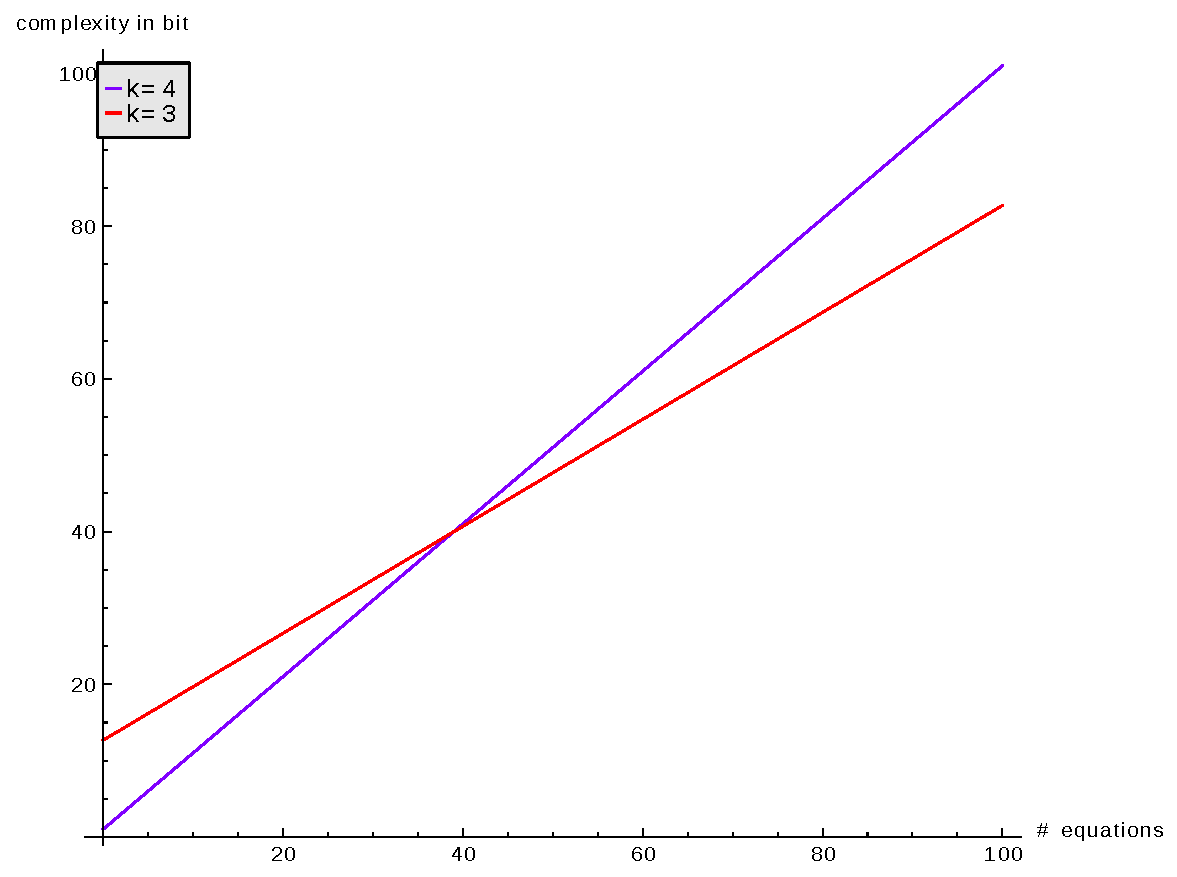
\includegraphics[width=10cm]{figures/hybridF5_vs_m_gf2.pdf}
\caption{Complexity of solving overdetermined random systems over $\mathbb{F}_2$ with HybridF5}
\label{fig:overgf2}
\end{figure}

\begin{figure}
\centering
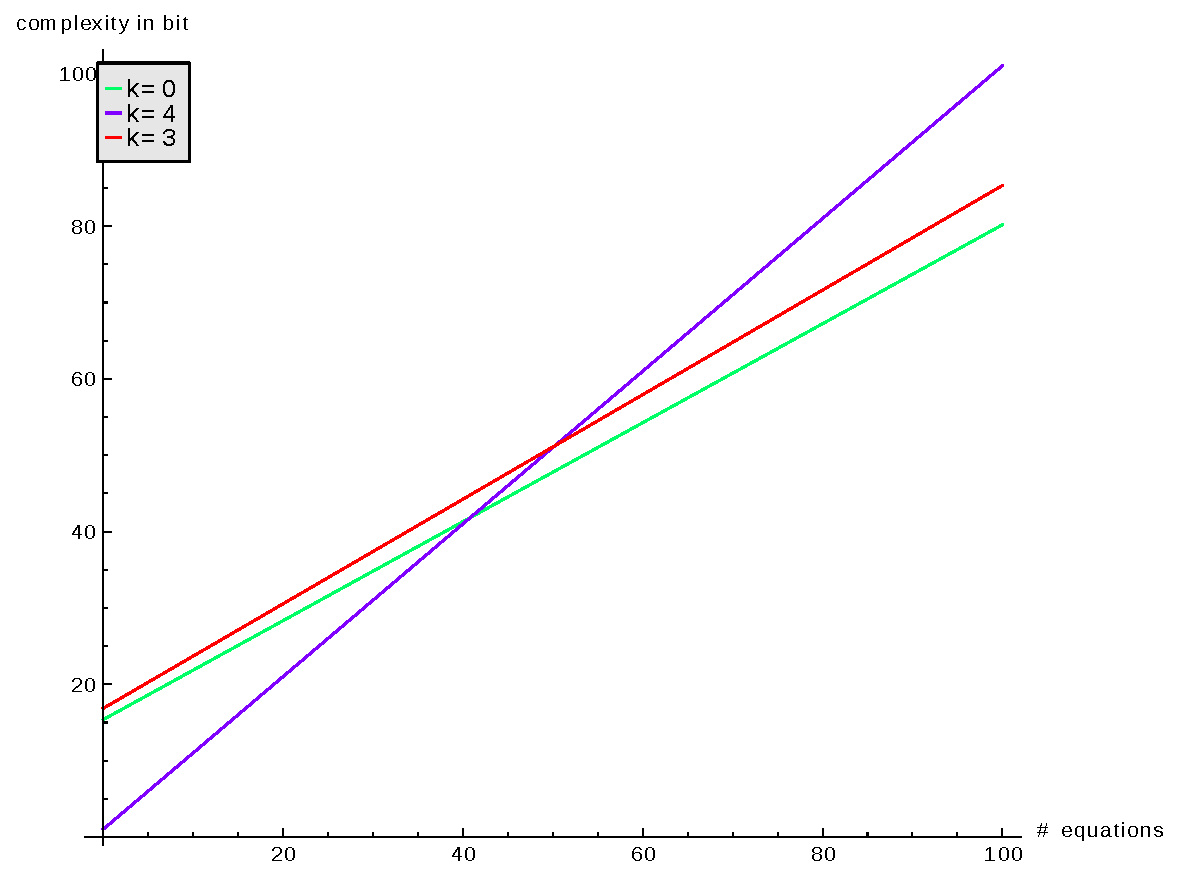
\includegraphics[width=10cm]{figures/hybridF5_vs_m_gf4.pdf}
\caption{Complexity of solving overdetermined random systems over $\mathbb{F}_4$ with HybridF5}
\label{fig:overgf4}
\end{figure}

\begin{figure}
\centering
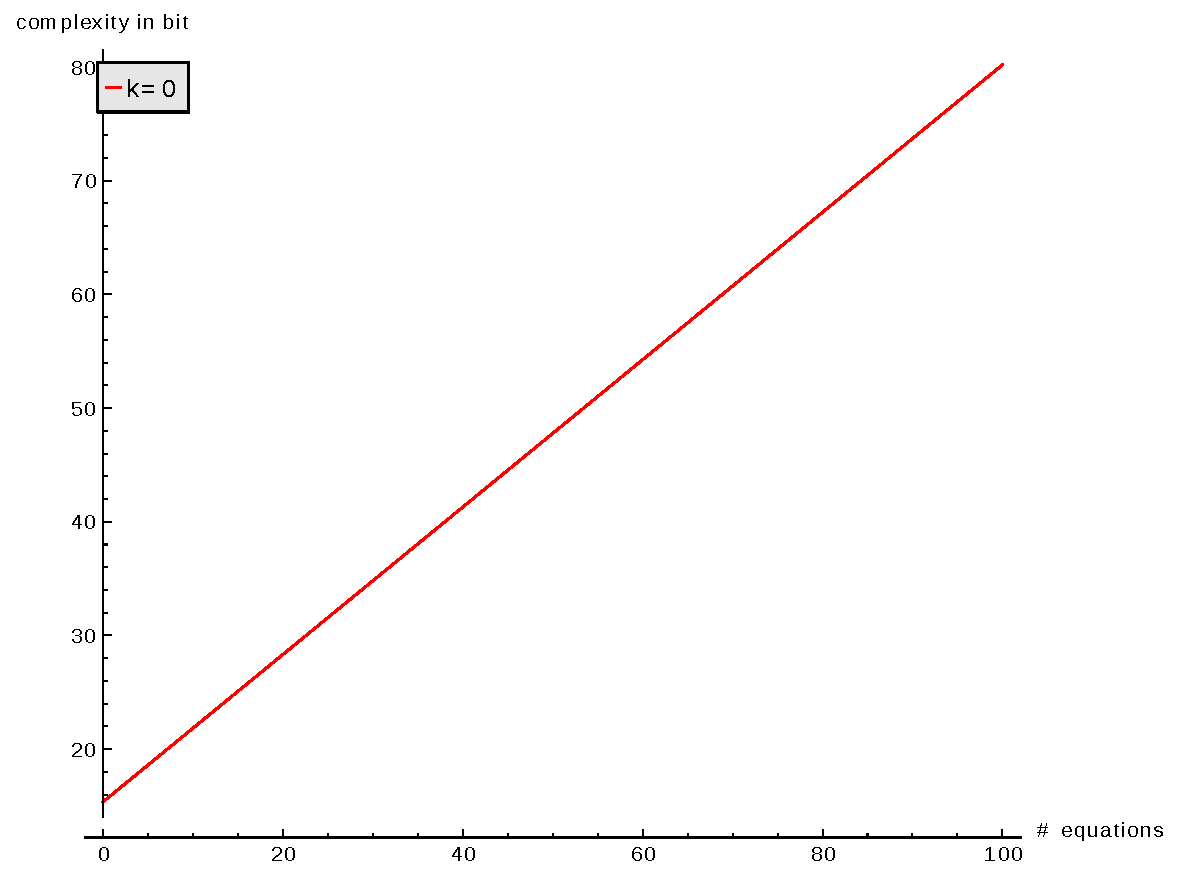
\includegraphics[width=10cm]{figures/hybridF5_vs_m_gf16.pdf}
\caption{Complexity of solving overdetermined random systems over $\mathbb{F}_{16}$ with HybridF5}
\label{fig:overgf16}
\end{figure}


\begin{figure}
\centering
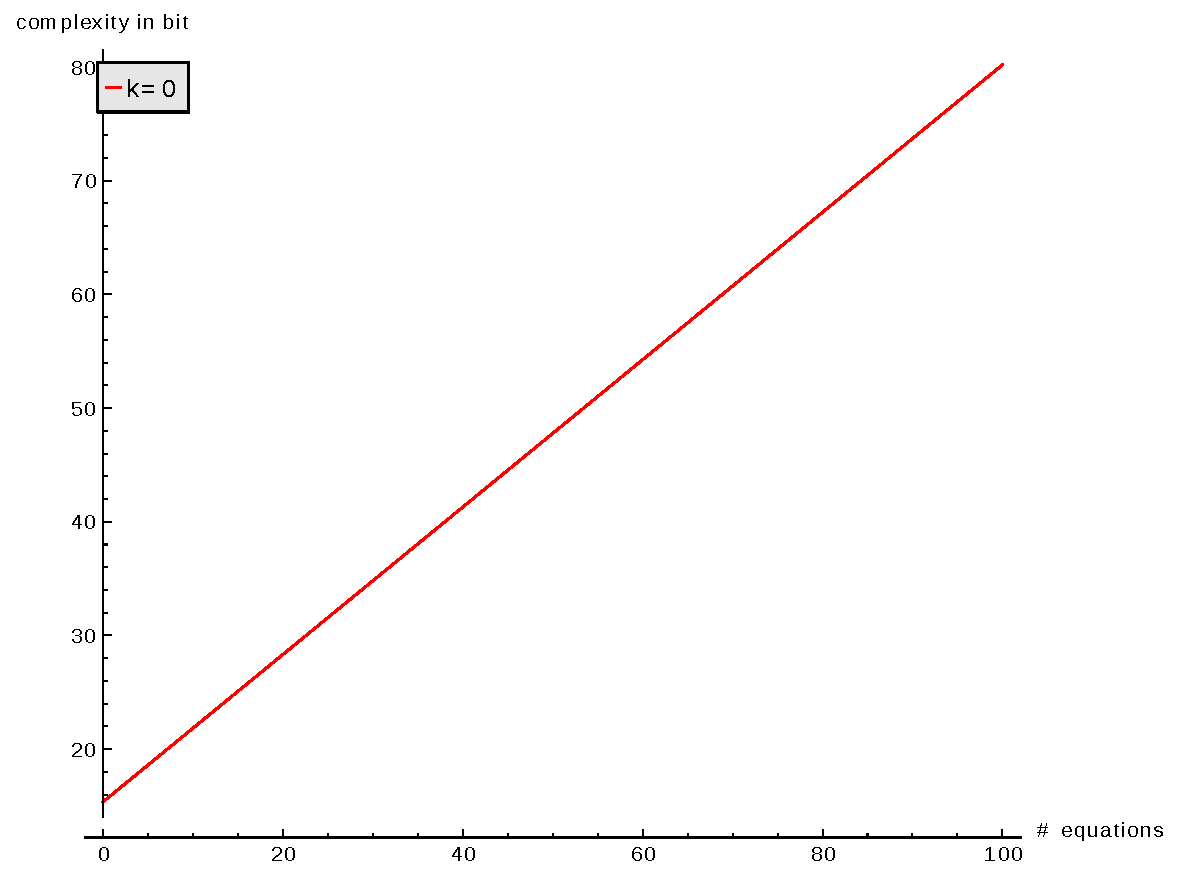
\includegraphics[width=10cm]{figures/hybridF5_vs_m_gf256.pdf}
\caption{Complexity of solving overdetermined random systems over $\mathbb{F}_{256}$ with HybridF5}
\label{fig:overgf256}
\end{figure}
A natural question in this context is to choose the best tradeoff, i.e. for which number $k\geq 0$ the complexity of the algorithm as shown by equation \eqref{eq:complexityHF5w} gets minimal. Guessing variables to build \textbf{overdetermined systems} reduces the complexity of each run of the F5 algorithm, but also increases the number of this runs. We found

\begin{itemize}
\item for overdetermined systems over $\mathbb{F}_{2}$ it is the best strategy to guess $7$ ($m\leq 41$), $6$ ($m\geq 42$),
\item for overdetermined systems over $\mathbb{F}_{4}$ it is the best strategy to guess $4$ ($m\leq 40$), $0$ ($m\geq 41$),
\item for overdetermined systems over $\mathbb{F}_{16}$ and $\mathbb{F}_{256}$ it is the best strategy to guess $0$ ($m>0$).
\end{itemize}

Evaluating \eqref{eq:complexityHF5w} for $m \in \left\{8,\cdots,108\right\}$, we find that the bit complexity of solving a overdetermined random system  of $m$ multivariate quadratic equations and $n$ variables using the HybridF5 algorithm is roughly
\begin{equation}
m+1
\label{eq:HF5_gf2_4}
\end{equation}
for systems over $\mathbb{F}_2$ and $\mathbb{F}_4$,
\begin{equation}
0.65\cdot m+15.36
\label{eq:HF5_gf16}
\end{equation}
for systems over $\mathbb{F}_{16}$,
\begin{equation}
0.65\cdot m+15.36
\label{eq:HF5_gf256}
\end{equation}
for systems over $\mathbb{F}_{256}$.
%. [] found a improved of the last bound saying that if the system has $(n \approx m^2/2)$ variables then the system can be solved again in polynomial time
%(thats why we have to increase the number of equations in UOV by 2).




%The case of determined system are studied in [Albrecht Thesis]. Because solve undetermined system are hardness than determined system, then the study of [] serve to signature schemes as UOV, Rainbow. Compared to determined systems, overdetermined systems are easy to solve with HybridF5. Hence, it is necessary recalculates new parameters for the minimal number of equations to defend multivariate scheme, that use overdetermined systems, against this attack.


%Since, there are independent attacks for each MPQCs, we have to use there result with the independly attacks to perform this analysis for each scheme separately. This analysis is perfom the the Chapter 6.
\chapter{{Some Multivariate Schemes}}
\label{chapter:back_ground_mpqc}
In chapter \ref{chap:mpqc}, we will analyse the security of some promising multivariate schemes using SAT solvers. But first we review how their algorithms and their known best attacks. 
\section{UOV Scheme}
The Unbalanced Oil Vinegar (UOV) scheme was proposed by \citet{Kipnis1999} and it is a generalisation of the original Oil and Vinegar scheme proposed by \citet{Patarin1997}. This scheme has not the usual standard construction, later we will explain this fact.

The polynomial map $P$ of UOV is defined has the following form:

\begin{equation}
 P=\left(\begin{matrix}
    p^{(1)}(\overset{v}{x_1},\cdots,\overset{v}{x_{n-m}},\overset{o}{x_{n-m+1}} \cdots,\overset{o}{x_n})  \\   
    \vdots \\
p^{(m)}(\overset{v}{x_1},\cdots,\overset{v}{x_{n-m}},\overset{o}{x_{n-m+1}} \cdots,\overset{o}{x_n})  \\ 
   \end{matrix}\right).
\label{eq:uov}
\end{equation}

In this context, $n$ is the number of variables and $m$ the number of equations of the polynomial map $P$. The variables $x_i$ for $1 \leq i \leq n-m$ are called of vinegar and are represented with the symbol $v$ over these variables. The variables $x_i$ where $n-m + 1 \leq i \leq n$ are called of oil and are represented with the symbol $o$ over these variables. The polynomials functions $p^{(i)}$ are defined as follow
$$p^{(i)} =\displaystyle\sum_{j=1}^{n-m}\displaystyle\sum_{k=1}^{n-m} \gamma_{j,k}^{i}\overset{v}{x_j}\overset{v}{x_k}+\displaystyle\sum_{j=1}^{n-m}\displaystyle\sum_{k=n-m+1}^{n} \gamma_{j,k}^{i}\overset{v}{x_j}\overset{o}{x_k}+\displaystyle\sum_{k=1}^{n-m} \beta_{k}^{i}\overset{v}{x_k}+\displaystyle\sum_{k=n-m+1}^{n} \beta_{k}^{i}\overset{o}{x_k}+\alpha^i.$$

Note that the vinegar variables are combined quadratically, whereas the oil variables are only combined with vinegar variables. Hence, replacing the vinegar variables with values in $\mathbb{F}_q$ is possible to obtain a linear system of $m$ equations in $n-m$ oil variables. That linear system can be resolved using the Gaussian elimination method easily. Besides, note that because we have the term $n-m$ this scheme can be used only for signature.\\
\noindent
\textit{Key Generation.} The UOV scheme ignore the usual linear transformation $S\in \mathbb{F}_q^m\rightarrow \mathbb{F}_q^m$ of the standard construction. This omission is because in UOV scheme all equations have the same shape, then is not necessary to hide some special structure. 

Therefore, the key generation processes works as follow. Select a invertible map $T\in \mathbb{F}_q^n\rightarrow \mathbb{F}_q^n$ and compute $\bar{P} = P \circ T$. Then the public key is $\bar{P}$ and the private key are $P$ and $T$.\\
\noindent
\textit{Signature Generation} To sign a document $d$ we use a hash function $H$ and compute $\boldsymbol h=H(d)$. After that, we compute $\boldsymbol y = P^{-1}(\boldsymbol h)$. Hence, the signature of the document $d$ is $\boldsymbol x = T^{-1}(\boldsymbol y)$. Note that $P^{-1}$ not means it be an invert map of $P$ but, one that find pre-images of $P$.\\
\noindent
\textit{Verification}
To verify that $\boldsymbol x$ is the signature of the document $d$, we compute $\boldsymbol h=H(d)$ and after one we compute $\boldsymbol h' = \bar{P}(\boldsymbol x)$. If $h' = h$ then the signature is verified, otherwise rejected.
\subsection{Known Best Attack against the UOV scheme}
According [thesis Albrecht] the  relevant attacks are the direct attack, the UOV attack of Kipnis and Shamir and the UOV Reconciliation attack. There is another attack proposed by called The Rainbow Band Separation attack is actually an extension of the UOV Reconciliation attack which uses the special structure of Rainbow; it is not suitable for UOV.

All three attacks (UOV, UOV Reconciliation and Rainbow Band Separation) find an equivalent private key, i.e  UOV/Rainbow private maps which compose to the same public key. However, in the case of UOV, this private key consists only of a UOV central map and one linear transformation, whereas in the case of Rainbow you have, besides the central map, two linear transformations. Therefore, the UOV and the UOV Reconciliation attack output two, whereas the Rainbow central map outputs three maps. Therefore the first two attacks can only be used against UOV, while the third one is used against Rainbow. 

Regarding the efficiency of the attacks: The UOV Reconciliation attack has hardly effect on the parameter choice of UOV. The reason for this is that it requires the solution of a multivariate quadratic system in $o$ equations (just as a direct attack). It is therefore not more efficient than a direct attack against UOV.

The UOV attack has a complexity of $O(q^{v-o})$, where q is the cardinality of the underlying field. To defend UOV against this attack, the difference between $v$ and $o$ should not be too small. If $v=o$, the attack runs in polynomial time and the scheme offers no security at all. To be on the conservative side, on therefore chooses the parameters of UOV to be $v >= 2o$.

To find good parameters for UOV, one first selects the number of equations in such a way that a direct attack against the scheme is infeasible (for $q=256$, this leads to $o = 28$). After this, to be secure against the UOV attack, one chooses $v=2o$. The number of variables in the scheme is therefore given by $n=o+v=3o$.
\section{Rainbow Scheme}
\section{STS Schemes}
The step-wise Triangular Schemes (STS) have a standard construction and were proposed by \cite{Wolf2005} as a generalization of the TPM schemes proposed by  \cite{Goubin:2000:CTC:647096.716863}.

\section{ABC Scheme}
This scheme has a standard construction and was proposed by \citet{Tao2013}. In the original paper there are mistakes in the decryption process. These mistakes has been addressed by \citet{Ding2014},  \citet{Tao2015} and by \citet{Petzoldt2016}. Here we will explain the ABC scheme with the modification of \citet{Petzoldt2016} which solve these mistakes. 

The main idea of this scheme is create matrices with high rank and use some Simple Matrix Multiplication to construct the map of polynomial functions $P$. Let $\mathbb{F}_q$ be a finite field. Let $s$ be a integer. Let $n=s^2$ a number of variables and $m=2n$ a number of equations of the map. Let $A$ be a matrix with dimensions $s\times s$ such that its entries are indeterminate belonging to $\mathbb{F}_q$. Let $B$ and $C$ be matrices with dimensions $s\times s$ such that its entries are multivariate polynomials of degree one . Define $E_1 = AB$ and $E_2 = AC$. Let $p^{({(i-1)}s+j)}$ and $p^{({s^2+(i-1)s+j})}$ be respectively the $(i,j)$ element of $E_1$ and $E_2$ respectively, where $(i,j=1,\cdots,s)$. Then each polynomial function of the polynomial map $P$ is define by the entries of $E_1$ and $E_2$ in the following way.

\begin{equation}
 P=\left(\begin{matrix}
    p^{(1)}(x_1,x_2,\cdots,x_n)  \\
    \vdots \\
    p^{(s^2)}(x_1,x_2,\cdots,x_n) \\
    p^{(s^2+1)}(x_1,x_2,\cdots,x_n) \\    
    \vdots \\
    p^{(m)} (x_1,x_2,\cdots,x_n) 
   \end{matrix}\right).
\label{eq:abc}
\end{equation}
\noindent
\textit{Key Generation.} Choose two invertible $s\times s$ matrices $T_1$ and $T_2$ and define $T=T_1 \otimes T_2$. Then, the public key, that is, the map $\bar{P}$, is constructed by using two affine transformations  $S\colon\mathbb{F}_q^{m}\rightarrow \mathbb{F}_q^{m}$ and $T\colon\mathbb{F}_q^{n}\rightarrow \mathbb{F}_q^{n}$ in the following way $\bar{P} = S \circ P \circ T$ and the private key consists of $T_1$, $T_2$, $B$, $C$, and $S$.\\
\noindent
\textit{Encryption.} To encrypt a message $\boldsymbol m \in \mathbb{F}^*$ there are 3 steps:
\begin{itemize} 
\item Split the message in blocks of size $n$, namely $m_1, m_2, m_3, \cdots$. 
\item After one, verify if the associate matrix $A$ of $m_1$ is invertible. If that matrix is invertible then we evaluate this message in the map $\bar{P}$, i.e. compute the ciphertext $\boldsymbol c_1 = \bar{P}(\boldsymbol m_1)$. Otherwise, Add some constant character to the block $m_1$ at random position and verify if the new associated matrix has inverse. 
\item We repeat the last step until the associated matrix has inverse and for all blocks of the message $\boldsymbol m$.\\
\end{itemize}
\noindent
\textit{Decryption.} The decryption process of the ciphertext $\boldsymbol c \in \mathbb{F}^n$ consists of four steps:
\begin{itemize}
\item[1] Compute $\boldsymbol x=S^{-1}(\boldsymbol c)$. The elements of the vector $\boldsymbol x\in \mathbb{F}^m$ are written into matrices $\bar{E}_1$ and $\bar{E}_2$ as follows 

\begin{equation}
 E_1=\left(\begin{matrix}
    x_1 & \cdots & x_s\\
    \vdots & & \vdots \\
    x_{(s-1)s+1} & \cdots & x_n 
   \end{matrix}\right), 
    E_2=\left(\begin{matrix}
    x_{n+1} & \cdots & x_{n+s}\\
    \vdots & & \vdots \\
    x_{n+(s-1)s+1} & \cdots & x_m 
   \end{matrix}\right).
\label{eq:2}
\end{equation}
\item[2] After one, it is necessary to compute the pre-image $\boldsymbol y$ of the system $\boldsymbol x=P(\boldsymbol y)$. To do this, there are four cases, namely:
\begin{itemize}
\item[-] If $\bar{E}_1$ is invertible, we consider the equation $B\bar{E}_1^{-1}\bar{E}_2-C=0$. Thus, we gets $n$ linear equations in the $n$ variables $y_1, \cdots, y_n$.
\item[-] If $\bar{E}_1$ is not invertible, but  $\bar{E}_2$, we consider $C\bar{E}_2^{-1}\bar{E}_1-B=0$. Thus, we gets $n$ linear equations in the $n$ variables $y_1, \cdots, y_n$.
\item[-] If neither $\bar{E}_1$ nor $\bar{E}_2$ are not invertible but $\bar{A}=A(\boldsymbol y)$ is invertible, we consider the relations $\bar{A}^{-1}\bar{E}_1-B=0$ and $\bar{A}^{-1}\bar{E}_2-C=0$. We interpret the elements of $A^{-1}$ as new variables $w_1, \cdots, w_n$ and therefore we gets $m$ linear equations in $m$ variables $w_1, \cdots, w_n, y_1, \cdots y_n$.
\end{itemize}
\item[3] Finally, we compute the plaintext by $\boldsymbol m = T^{-1}(y1, \cdots , yn)$. 
\item[4] After having found the encrypted plaintext $m$, we remove all the appearances of
the constant character to get the original message.
\end{itemize} 
%Investigar the best know attacks against ABC
%Como clasificar los ataques? structurales? structural key recovery attack?
\subsection{Known Best Attack against the ABC scheme}
%talk about Know best attack doesnot matter memory,
There are several attacks that it is possible to apply against several multivariate schemes. Among them, there is  the Minrank attack proposed by against the multivariate proposed by and called HFE. 
 
\citet{Moody2014} developed a attack, which combined with the Minrank attack is the known best attack against the ABC scheme.

Below, we will explain first the Minrank attack against the ABC scheme and after the strategy proposed by \citet{Moody2014}.\\
\noindent
\textbf{Minrank Attack Against the ABC Scheme}\\
\noindent
\textbf{An Asymptotically Optimal Structural Attack on the ABC Scheme}

\part{Contributions}
\chapter{{Hash-Coding Based Cryptography}}
\section{One-Time Signatures}
\section{Merkle Scheme}
\subsection{Security of the Merkle Scheme}

\section{Modified Scheme}
\label{sec:modified_scheme}
\[
	\sigma_{j}^i=(i,j,\normalfont\textsf{V}_j^i,\sigma_{\textsc{SeedBMOTS}},\overbrace{(a_0,\cdots,a_{h-1})}^{A_j^i}).
\]

\subsection{Security Analysis}
\subsection{Costs}
\subsubsection{Complexity}
Key Generation
Signature Generation
Signature Verify


\subsubsection{Sizes}

\textbf{Keys Size.}
Remember that the private key is a set consisting of 
1) the seeds $\textsc{SeedBMOTS}^0_0$ and $\textsc{SeedBMOTS-J}_j^i$ used to generate the private keys of the modified BMOTS instances and 2) two seeds, $\textsc{SeedPL}^0_u$ and $\textsc{SeedPL}^0_l$ used to generate $e^i_j$. Then, the maximum size of a private key of our propose is

\begin{equation}
\begin{split}
    S_{sk} &= \iota + n + N' + N''
\end{split}
\end{equation}
As we seen, a public key of our propose consisting of: 1) The root of the modified Merkle tree and 2) a $N$-bit seed $\textsc{SeedH}$. Then, the maximum size of a public key of our propose is
\begin{equation}
\begin{split}
    S_{pk} &= n + N
\end{split}
\end{equation}
\textbf{Signature Size.} To compute the signature size, we are going to calculate the number of bits occupied by each its component. Remember that a signature has the following components

\[
	\sigma_{j}^i=(i,j,\normalfont\textsf{V}_j^i,\sigma_{\textsc{BMOTS}},\overbrace{(a_0,\cdots,a_{h-1})}^{A_j^i}).
\]

$i$ and $j$ are integers and, we are going to represent the size of a integer as $S_{int}$. Since $\sigma_{\textsc{BMOTS}}$ is $|(h,c)|$, then the maximum size of this component is given by:
\begin{equation}
S_{\textsc{BMOTS}} = k + \ln{{N}\choose{2n}} + \ln(2n)
\label{chap:7:eq:c_sig}
\end{equation}
where $\ln{{N}\choose{2n}} + \ln(2n)$ is the size of $c$, when $c$ is representing as its rank in some conventional ordering of binary string and its weights. 
It is clear that the size of $\normalfont\textsf{V}_j^i \in \mathbb{F}_2^{R\times k}$ is $kR$. The size of each node in the modified Merkle tree is $k$, then the size of $A_j$ is $hk$. Thus, the size of a signature of our propose is:

\begin{equation}
\begin{split}
    S_{sig} &= 2S_{int} + S_{\textsc{BMOTS}} + kR + hk\\
    &= 2S_{int} + k + \ln{{N}\choose{2n}} + \ln(2n) + kR + hk\\
    &= 2S_{int} + k(h+R+1) + \ln{{N}\choose{2n}} + \ln(2n)
\end{split}
\end{equation}

%Why can I sign 2^\lamda/2 documents (using the BMOTS parameters)
%The annswer of this question is in Postquatum Book (Security of MSS)

\subsection{Choosing Parameters}
As we seen in section \ref{section:modified_scheme}, the number of documents that it is possible to sign using one syndrome is equal to the number of solutions of the follow random linear system 

\begin{equation}
     \normalfont\textsf{C} \boldsymbol{e^i_x} = \boldsymbol{s}^i_l.
     \label{eq:cxs}
\end{equation}

Let $t$ the number of solutions of the system above. To take advantage of the original Merkle system is necessary that at least $t>2$. Known results about finite fields suggest to use undetermined systems, since they have several solutions with high probability. In particular, we choose full rank matrices to construct that systems because the probability is greater than others. The number of $R''\times N''$ matrices over $\mathbb{F}_2$ that have rank $R''$ is

\begin{equation}
G(R'',N'',r) = {N'' \brack r}_2\sum_{l=0}^{r}(-1)^{r-l}{r \brack l}_22^{R''l+{r-l \choose 2} }
\label{eq:number_matrices}
\end{equation}
where ${N'' \brack r}_2$ and ${r \brack l}_2$ are Gaussian coefficients.

Let $\Pr(R'',N'',r)$ the probability that a $R''\times N''$ matrix has rank $r$. To find this probability it is only necessary to divide \eqref{eq:number_matrices} by the total number of $R''\times N''$ matrices, that is 
\begin{equation}
\Pr(R'',N'',r) = \dfrac{G(R'',N'',r)}{2^{R''N''}}   
\end{equation}


As in all fields, if the matrix of the system and the augmented matrix have same rank $r(r\leq N'')$, the set of solutions is an affine subspace of $F^{N''}_2$ of co-dimension $r$, hence there are $t=2^{N''-r}$ points in this subspace. If the rank of the augmented matrix is greater than the rank of the matrix of the system, there is no solution. 

Table \ref{table:suggested_parameters} shows suggested parameters for practical security levels. We choose the values $R', N', k$ and $n$ such that the BMOTS modified system resist the Otmani-Tillich attack. In addition, to construct the matrix $A$ we suggest using the same type of matrices used in [], that is, to use double-circulant parity check matrices, because these matrices define codes meeting the GV bound [7] with high probability. 

As we said, to construct $H$ we need still the matrix $B$ where $N''>R''$. Table \ref{table:suggested_parameters:B} shows suggested parameters for $B$. 


\begin{table}[]
\centering
\caption{Suggested parameters for standard security levels}
\label{table:suggested_parameters}
\begin{tabular}{|l|l|l|l|l|l|l|l|l|l|l|l|}
\hline
$\lambda$ & $k$ & $n$ & $R'=|A|$ & $N'$    & $l$ & $p$ & $E{|I|}$ & GV & $|V|$ & $|h,c|$ & Merkle tree \\ \hline
80        & 160 & 380   & 5000    & 10000  & 8   & 3   & 196.38   & 6  &  800000  &       &             \\ \hline
112       & 224 & 550   & 3700    & 7400   & 8   & 5   & 292.24   & 11 &     &       &             \\ \hline
128       & 256 & 630   & 9400    & 18800  & 8   & 5   & 323.85   & 11 &     &       &             \\ \hline
192       & 384 & 940   & 87500   & 175000 & 8   & 6   & 472.11   & 13 &     &       &             \\ \hline
256       & 512 & 1280  & 9450    & 18900  & 8   & 12  & 664.66   & 24 &     &       &             \\ \hline
\end{tabular}
\end{table}

\begin{table}[]
\centering
\caption{Suggested parameters for $B$}
\label{table:suggested_parameters:B}
\begin{tabular}{|l|l|l|l|}
\hline
$t$ & $R''$ & $N''$ & $\Pr(R'',N'',r)$ \\ \hline
$64$ & $4$ & $10$ & $0.99$ \\ \hline
\end{tabular}
\end{table}

%J out of B
%$k in JM11 output size of hash 
%(N n) >= 2^\lamba
% Due to the random nature of the system \ref{eq:cxs}, we will calculate for which parameters that happens with high probability. Since these parameters affect the size of $ \normalfont\textsf{H}$, we need to found a trade-off relation between the number of documents that it is possible to sign and the size of $\normalfont\textsf{H}$. More formally, let $Rank$ a function that calculates the rank of a matrix. Let $\normalfont\textsf{C}:\boldsymbol{s}^i_l$ a notation to represent the augmented matrix of \eqref{eq:cxs}, then we need to calculate:
% \begin{equation}
%      P = \Pr[Rank(\normalfont\textsf{C}) = R''-\log(t) \wedge Rank(\normalfont\textsf{C}:\boldsymbol{s}^i_l) = R''-\log(t)]
%      \label{eq:cxs_rank_probability}
% \end{equation}
% This probability can be easily calculated with know results, and in follow we will explain this in more detail. 


% The number of full rank matrices $a \times b$, with $a \geq b$ is given by:

% \begin{equation}
%     F(a,b) = (2^a-1)(2^a-2)\cdots (2^{a}-2^{b-1}) = \prod_{i=0}^{b-1}(2^a-2^i)
% \end{equation}
% If $G(a,b,r)$ denotes the number of $a\times b$ matrices of rank $r$, then 
% \begin{equation}
% G(a,b,r) = \dfrac{F(b,r)F(a,r)}{F(r,r)}
% \end{equation}

% Let $\Pr(a,b,r)$ the probability that a $a\times b$ matrix has rank $r$. To find this probability it is only necessary to divide this quantity by the total number of $a\times b$ matrices, that is 
% \begin{equation}
% \Pr(a,b,r) = \dfrac{G(a,b,r)}{2^{ab}}   
% \end{equation}






% %%%%%%%%%%%%%%%%%%%%%%%%%%%%%%%%%%%%%%%%%%%%%%%%%%%%%%%%
% % If every $a\times b$ matrix is equally likely to occur, the probability of selecting a matrix with full rank is

% % \begin{equation}
% %     P(a,b) = 2^{-ab}F(a,b) = \prod_{i=0}^{b-1}(1-2^{i-a})
% % \end{equation}

 


% That is, we need to calculate 
% \begin{equation}
%     P(a,b,r)  = \Pr[Rank(\normalfont\textsf{C}) = R''-\log(t) \wedge Rank(\normalfont\textsf{C}:\boldsymbol{s}^i_l) = R''-\log(t)]
%      \label{eq:cxs_rank_probability}
% \end{equation}

% Before, to calculate that relation, we are going to estimate a relation to known the probability of random linear system \eqref{eq:cxs} to have $t$ solutions
% There are few known results about the number of solutions of random matrices that will be needed. Some further details can be found in [][]. 


% In our propose how many document, we can sign?
% 1.-What is a probability of random linear system over GF(2) Cx=s to have "so" solutions, for example 
% 2.-Trade-off number of solutions and public key size
% \subsection{Comparison}


\chapter{{Direct Attack on MQ using CDCL SAT solvers}}
\label{chap:MPQC}
%\section{Secure Parameters against HybridF5 attack}
In this chapter, we are going to review the best known structural attacks  against the ABC, UOV and Rainbow multivariate schemes. These known best structural attacks to each specific scheme together the HybridF5 attack given secure parameters which we are going to use to construct several instances of these schemes and attack them using CDCL SAT solvers. 

Specifically, we used a massively parallel portfolio SAT solver called HordeSAT which used MPI. As we said, the SAT solvers in the portfolio can be instances of a single solver with different configuration settings. Additionally the solvers can exchange information usually in the form of clauses.
\section{UOV}
Taking into account the attack of \cite{Thomae2012} and using the equations \eqref{eq:complexdetermined_gf16},\eqref{eq:complexdetermined_gf31} and \eqref{eq:complexdetermined_gf256} \cite{AlbrechtPetzoldt2013} has calculated the secure parameters for the Rainbow and UOV schemes. Because of the attack of \cite{Thomae2012} reduce the number of equations in the public systems by 2 before applying an algorithm like HybridF5, \cite{AlbrechtPetzoldt2013} increased the number of equations by 2. Besides, to defend the scheme against the
UOV attack of \cite{Kipnis1999}, they recommend choose $v=2\cdot o$. Thus, in the Table \ref{table:security_level_uov} are shown the proposed parameter sets for the UOV scheme for different levels of security and different underlying fields.

\begin{table}
\centering
\caption{UOV parameters and security level for $\mathbb{F}_{16}$, $\mathbb{F}_{31}$ and $\mathbb{F}_{256}$}
\label{table:security_level_uov}
\begin{tabular}{|c|c|c|c|c|c|c|}
\hline
\multicolumn{1}{|c|}{}                     & \multicolumn{2}{c|}{$\mathbb{F}_{16}$}            & \multicolumn{2}{c|}{$\mathbb{F}_{31}$}            & \multicolumn{2}{c|}{$\mathbb{F}_{256}$}           \\ \hline
\multicolumn{1}{|c|}{security level (bit)} & \multicolumn{1}{c|}{$o$} & \multicolumn{1}{c|}{$v$} & \multicolumn{1}{c|}{$o$} & \multicolumn{1}{c|}{$v$} & \multicolumn{1}{c|}{$o$} & \multicolumn{1}{c|}{$v$} \\ \hline
16 & 3 & 6 & 3 & 6 & 3 & 6 \\ \hline
17 & 3 & 6 & 4 & 8 & 4 & 8 \\ \hline
18 & 4 & 8 & 4 & 8 & 4 & 8 \\ \hline
19 & 4 & 8 & 4 & 8 & 5 & 10 \\ \hline
20 & 4 & 8 & 5 & 10 & 5 & 10 \\ \hline
21 & 5 & 10 & 5 & 10 & 5 & 10 \\ \hline
22 & 5 & 10 & 6 & 12 & 6 & 12 \\ \hline
23 & 6 & 12 & 6 & 12 & 6 & 12 \\ \hline
24 & 6 & 12 & 6 & 12 & 6 & 12 \\ \hline
25 & 7 & 14 & 7 & 14 & 7 & 14 \\ \hline
26 & 7 & 14 & 7 & 14 & 7 & 14 \\ \hline
27 & 7 & 14 & 8 & 16 & 8 & 16 \\ \hline
28 & 8 & 16 & 8 & 16 & 8 & 16 \\ \hline
29 & 8 & 16 & 8 & 16 & 8 & 16 \\ \hline
30 & 9 & 18 & 9 & 18 & 9 & 18 \\ \hline
31 & 9 & 18 & 9 & 18 & 9 & 18 \\ \hline
32 & 10 & 20 & 10 & 20 & 10 & 20 \\ \hline
33 & 10 & 20 & 10 & 20 & 10 & 20 \\ \hline
34 & 11 & 22 & 10 & 20 & 10 & 20 \\ \hline
35 & 11 & 22 & 11 & 22 & 11 & 22 \\ \hline
36 & 11 & 22 & 11 & 22 & 11 & 22 \\ \hline
37 & 12 & 24 & 12 & 24 & 11 & 22 \\ \hline
38 & 12 & 24 & 12 & 24 & 12 & 24 \\ \hline
39 & 13 & 26 & 12 & 24 & 12 & 24 \\ \hline
40 & 13 & 26 & 13 & 26 & 13 & 26 \\ \hline
41 & 14 & 28 & 13 & 26 & 13 & 26 \\ \hline
42 & 14 & 28 & 14 & 28 & 13 & 26 \\ \hline
43 & 14 & 28 & 14 & 28 & 14 & 28 \\ \hline
44 & 15 & 30 & 14 & 28 & 14 & 28 \\ \hline
\end{tabular}
\end{table}

\noindent
\textbf{Solving UOV intances over $\mathbb{F}_{16}$ using CDCL SAT solvers}
\begin{table}[]
\centering
\caption{HordeSAT configurations}
\label{my-label}
\begin{tabular}{lccccc}
\hline
\multicolumn{1}{l|}{Core Solvers} & \multicolumn{1}{c|}{Parallel Solved} & \multicolumn{1}{c|}{Avg.} & \multicolumn{1}{c|}{Tot.} & \multicolumn{1}{c}{Med} \\ \hline
solved-lingeling\_uov\_1x6x4 & 150 & 1 & 1.00 & 1.00 \\\hline
solved-lingeling\_uov\_2x6x4 & 150 & 3 & 1.68 & 1.12  \\\hline
solved-lingeling\_uov\_4x6x4 & 150 & 4 & 2.15 & 1.49 \\\hline
solved-lingeling\_uov\_8x6x4 & 150  & 14 & 6.39 & 2.83 \\\hline
solved-lingeling\_uov\_16x6x4 & 150  & 13 & 11.70 & 2.45  \\\hline
solved-lingeling\_uov\_32x6x4 & 150 & 12 & 17.46 & 2.86 \\\hline
solved-lingeling\_uov\_64x6x4 & 150 & 15 & 20.64 & 2.36 \\\hline
solved-lingeling\_uov\_128x6x4 & 150 & 19 & 25.22 & 2.10 \\\hline
solved-lingeling\_uov\_256x6x4 & 150  & 10 & 14.41 & 1.33  \\\hline
solved-lingeling\_uov\_512x6x4 & 150  & 18 & 21.37 & 1.36  \\\hline
\end{tabular}
\end{table}



\section{ABC}
Following the model showed in \cite{AlbrechtPetzoldt2013} we have calculated the secure parameters for the ABC scheme proposed by \cite{Tao2015}. Taking into account that the attack of \cite{Thomae2012}  reduce the number of equations in the public systems by 2 before applying an algorithm like HybridF5, we increased the number of equations by 2. Also, the known best structural attack against this scheme was proposed by \cite{Moody2014} and its complexity is 
\begin{equation}
s^6\cdot q^{s+4}
\label{eq:structural}
\end{equation}
for even characteristic and 
\begin{equation}
s^6\cdot q^{s+2}
\end{equation} for odd characteristic. 
%In this thesis, we have to study secure parameters of the ABC scheme constructed over finite fields with even characteristic.
Hereafter, we are going to name StructuralABC the attack proposed by \cite{Moody2014}. 

We use the equations \eqref{eq:complexityHF5w} and \eqref{eq:structural} to make a comparison between the complexity of the HybridF5 and StructuralABC attacks against instances of the ABC cryptosystem over $\mathbb{F}_2$, $\mathbb{F}_4$, $\mathbb{F}_{16}$ and $\mathbb{F}_{256}$. Figures \ref{fig:hybridF5_structural_gf2}, \ref{fig:hybridF5_structural_gf4}, \ref{fig:hybridF5_structural_gf16} and \ref{fig:hybridF5_structural_gf256} show the results when the equations \eqref{eq:complexityHF5w} and \eqref{eq:structural} are evaluated for $m \in \{8,\cdots,108\}$.\footnote{for the case of the HybridF5 was chose the minimum k - note by Juan}.

Clearly figure \ref{fig:hybridF5_structural_gf256} shows that the best attack is the HybridF5 for those values of $m$. However, in figures \ref{fig:hybridF5_structural_gf2}, \ref{fig:hybridF5_structural_gf4} and \ref{fig:hybridF5_structural_gf16} are showed that there is not a absolute best attack for those chosen values of $m$. Thus, to be more precise and determine which is the intersection point that define at which interval the best attack is HybridF5 or StructuralABC, we have to re-write the equations \eqref{eq:HF5_gf2_4}, \eqref{eq:HF5_gf16} and  \eqref{eq:HF5_gf256} for the critic intervals. Evaluating the equation \eqref{eq:complexityHF5w} for the critic values, we find that the bit complexity of the HybridF5 attack against instances of the ABC scheme with $m$ multivariate quadratic equations and $n$ variables is roughly
%GF2,GF4:m=1...7;GF16:m=18...24
\begin{equation}
0.72\cdot m+ 3.45
\end{equation}
for system over $\mathbb{F}_2$,
\begin{equation}
1.28\cdot m + 2.45
\end{equation}
for system over $\mathbb{F}_4$,
\begin{equation}
0.77\cdot m + 11.62
\end{equation}
for system over $\mathbb{F}_{16}$,

On other hand, evaluating \eqref{eq:structural} for $m\in \{8,\cdots,108\}$, we find that the bit complexity of the StructuralABC attack against instances of the ABC scheme with $m$ multivariate quadratic equations and $n$ variables is roughly
\begin{equation}0.15\cdot m + 14.56\label{eq:structuralgf2}\end{equation}
for system over $\mathbb{F}_2$,
\begin{equation}0.19\cdot m + 20.9\label{eq:structuralgf4}\end{equation}
for system over $\mathbb{F}_4$,
\begin{equation}0.29\cdot m + 33.42\label{eq:structuralgf16}\end{equation}
for system over $\mathbb{F}_{16}$,
\begin{equation}0.5\cdot m + 58.47\label{eq:structuralgf256}\end{equation}
for system over $\mathbb{F}_{256}$.

Thus, according this comparison, we find 
\begin{itemize}
\item for instances of the ABC scheme over $\mathbb{F}_2$ the known best attack is the HybridF5 attack, if  $m\leq 19$ and the StructuralABC if $m\geq 20$,
\item for instances of the ABC scheme over $\mathbb{F}_4$ the known best attack is the HybridF5 attack, if  $m\leq 17$ and the StructuralABC if $m\geq 18$,
\item for instances of the ABC scheme over $\mathbb{F}_16$ the known best attack is the HybridF5 attack, if  $m\leq 45$ and the StructuralABC if $m\geq 46$,
\item for instances of the ABC scheme over $\mathbb{F}_{256}$ the known best attack is the HybridF5 attack for all considered cases of $m$.
\end{itemize}

\begin{figure}
\centering
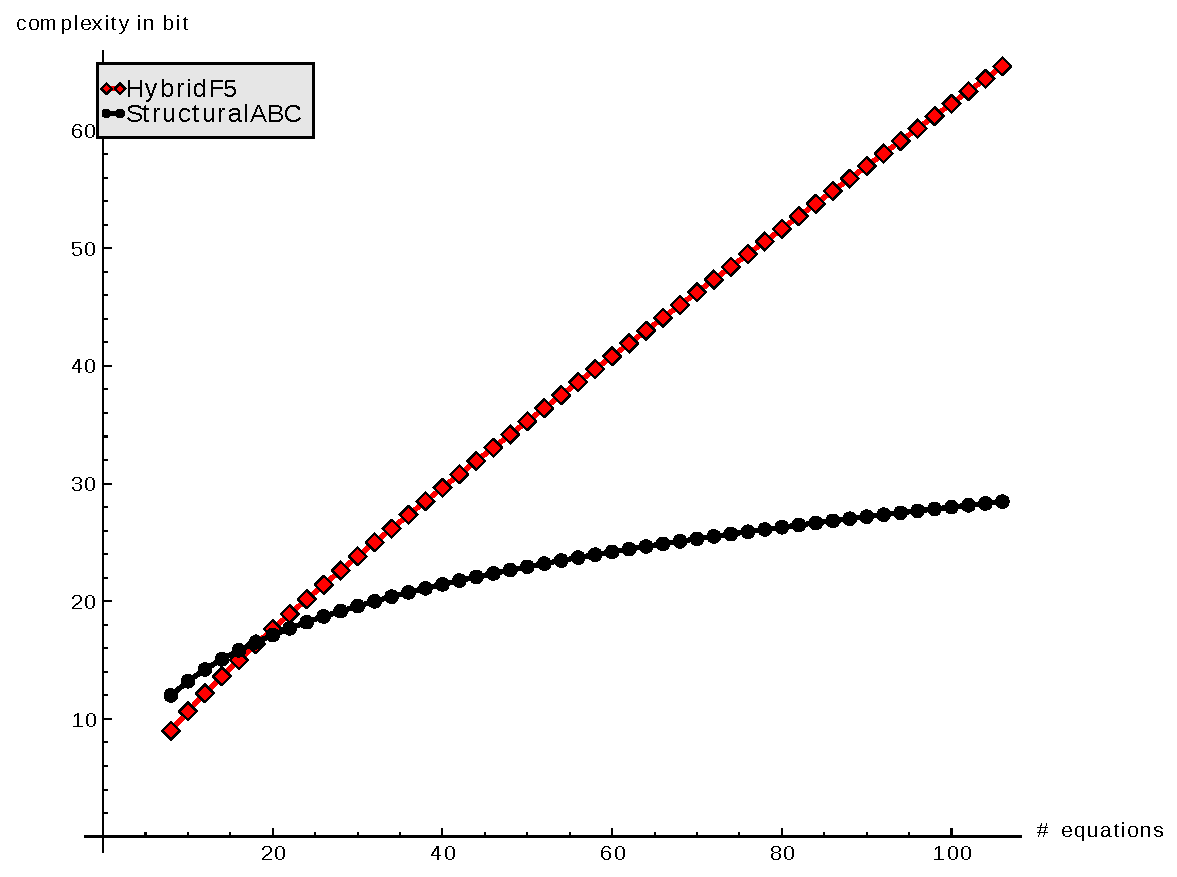
\includegraphics[width=10cm]{figures/hybridF5_structural_vs_m_gf2.pdf}
\caption{Complexity of the HybridF5 and StructuralABC attacks against instances of the ABC cryptosystem over $\mathbb{F}_2$.}
\label{fig:hybridF5_structural_gf2}
\end{figure}

\begin{figure}
\centering
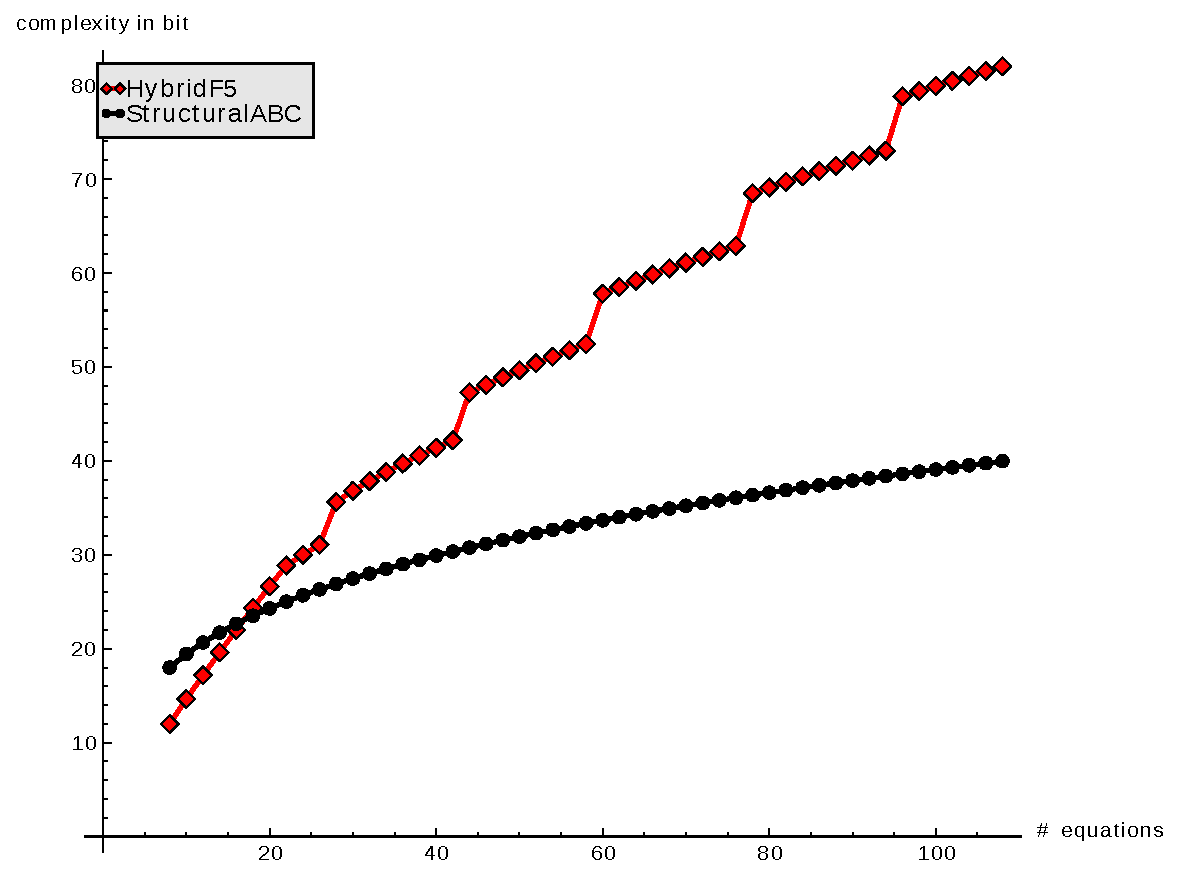
\includegraphics[width=10cm]{figures/hybridF5_structural_vs_m_gf4.pdf}
\caption{Complexity of the HybridF5 and StructuralABC attacks against instances of the ABC cryptosystem over $\mathbb{F}_4$.}
\label{fig:hybridF5_structural_gf4}
\end{figure}

\begin{figure}
\centering
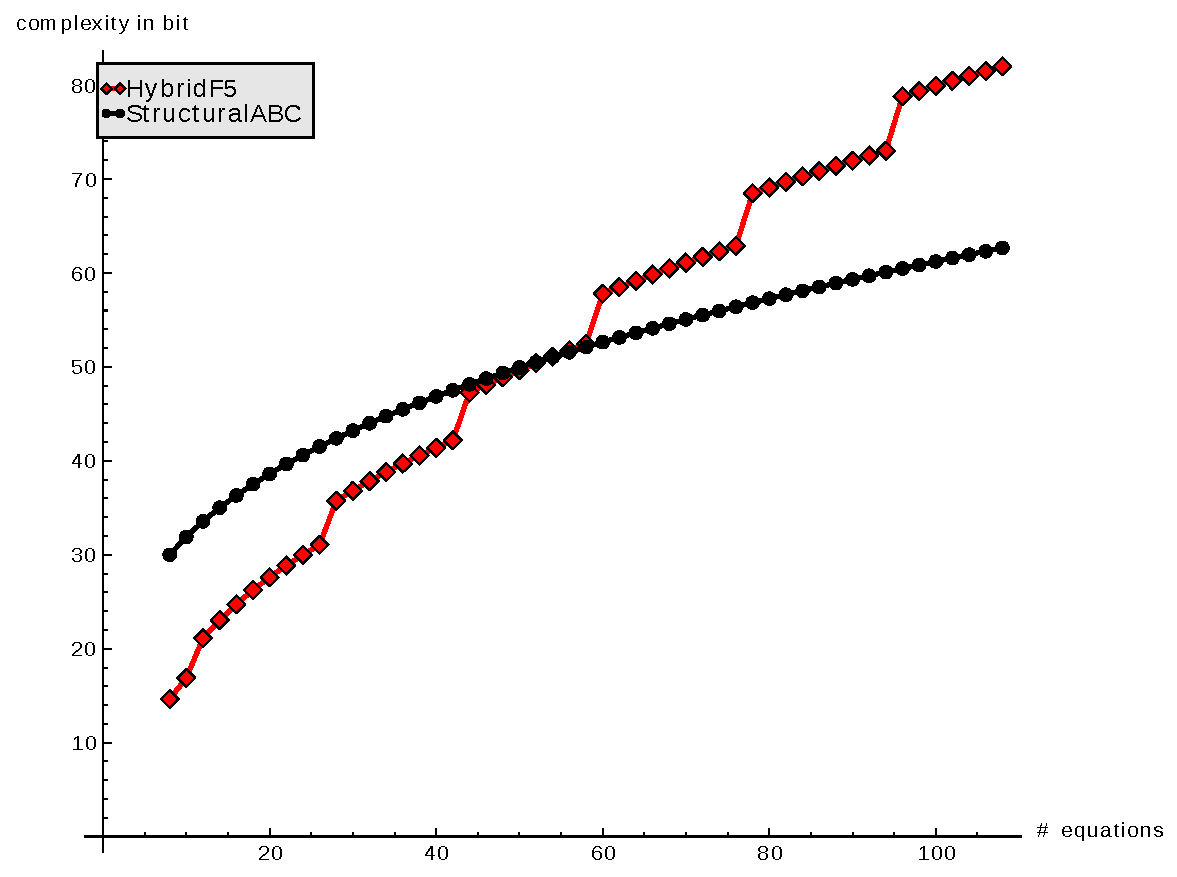
\includegraphics[width=10cm]{figures/hybridF5_structural_vs_m_gf16.pdf}
\caption{Complexity of the HybridF5 and StructuralABC attacks against instances of the ABC cryptosystem over $\mathbb{F}_{16}$.}
\label{fig:hybridF5_structural_gf16}
\end{figure}


\begin{figure}
\centering
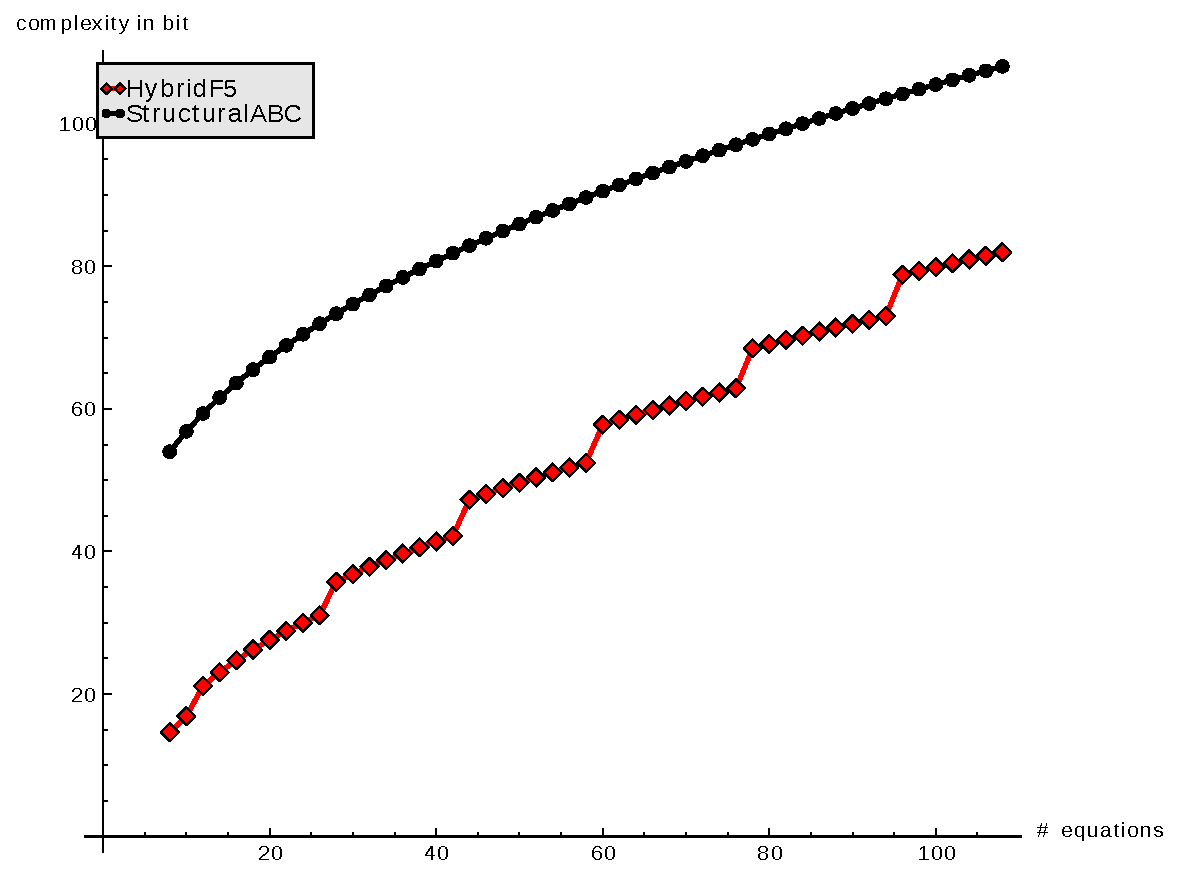
\includegraphics[width=10cm]{figures/hybridF5_structural_vs_m_gf256.pdf}
\caption{Complexity of the HybridF5 and StructuralABC attacks against instances of the ABC cryptosystem over $\mathbb{F}_{256}$.}
\label{fig:hybridF5_structural_gf256}
\end{figure}
In the Table \ref{table:security_level_abc} are shown the proposed parameter sets for the ABC scheme for different levels of security and different underlying fields.

\begin{table}[]
\centering
\caption{My caption}
\label{my-label}
\begin{tabular}{|c|c|c|c|c|}
\hline
                    & $\mathbb{F}_2$           & $\mathbb{F}_4$           & $\mathbb{F}_{16}$          & $\mathbb{F}_{256}$         \\ \hline
security level(bit) & \multicolumn{1}{c|}{$s$} & \multicolumn{1}{c|}{$s$} & \multicolumn{1}{c|}{$s$} & \multicolumn{1}{c|}{$s$} \\ \hline
16 &$\sqrt{ 10 }$&$\sqrt{ 7 }$&$\sqrt{ 4 }$&$\sqrt{ 3/2 }$\\ \hline
17 &$\sqrt{ 11 }$&$\sqrt{ 7 }$&$\sqrt{ 9/2 }$&$\sqrt{ 5/2 }$\\ \hline
18 &$\sqrt{ 13 }$&$\sqrt{ 7 }$&$\sqrt{ 5 }$&$\sqrt{ 3 }$\\ \hline
19 &$\sqrt{ 16 }$&$\sqrt{ 8 }$&$\sqrt{ 6 }$&$\sqrt{ 4 }$\\ \hline
20 &$\sqrt{ 19 }$&$\sqrt{ 8 }$&$\sqrt{ 13/2 }$&$\sqrt{ 9/2 }$\\ \hline
21 &$\sqrt{ 23 }$&$\sqrt{ 8 }$&$\sqrt{ 7 }$&$\sqrt{ 11/2 }$\\ \hline
22 &$\sqrt{ 26 }$&$\sqrt{ 9 }$&$\sqrt{ 15/2 }$&$\sqrt{ 6 }$\\ \hline
23 &$\sqrt{ 29 }$&$\sqrt{ 9 }$&$\sqrt{ 17/2 }$&$\sqrt{ 7 }$\\ \hline
24 &$\sqrt{ 33 }$&$\sqrt{ 10 }$&$\sqrt{ 9 }$&$\sqrt{ 15/2 }$\\ \hline
25 &$\sqrt{ 36 }$&$\sqrt{ 12 }$&$\sqrt{ 19/2 }$&$\sqrt{ 17/2 }$\\ \hline
26 &$\sqrt{ 39 }$&$\sqrt{ 15 }$&$\sqrt{ 21/2 }$&$\sqrt{ 9 }$\\ \hline
27 &$\sqrt{ 43 }$&$\sqrt{ 17 }$&$\sqrt{ 11 }$&$\sqrt{ 10 }$\\ \hline
28 &$\sqrt{ 46 }$&$\sqrt{ 20 }$&$\sqrt{ 23/2 }$&$\sqrt{ 21/2 }$\\ \hline
29 &$\sqrt{ 49 }$&$\sqrt{ 23 }$&$\sqrt{ 25/2 }$&$\sqrt{ 23/2 }$\\ \hline
30 &$\sqrt{ 53 }$&$\sqrt{ 25 }$&$\sqrt{ 13 }$&$\sqrt{ 25/2 }$\\ \hline
31 &$\sqrt{ 56 }$&$\sqrt{ 28 }$&$\sqrt{ 27/2 }$&$\sqrt{ 13 }$\\ \hline
32 &$\sqrt{ 59 }$&$\sqrt{ 30 }$&$\sqrt{ 14 }$&$\sqrt{ 14 }$\\ \hline
33 &$\sqrt{ 63 }$&$\sqrt{ 33 }$&$\sqrt{ 15 }$&$\sqrt{ 29/2 }$\\ \hline
34 &$\sqrt{ 66 }$&$\sqrt{ 36 }$&$\sqrt{ 31/2 }$&$\sqrt{ 31/2 }$\\ \hline
35 &$\sqrt{ 69 }$&$\sqrt{ 38 }$&$\sqrt{ 16 }$&$\sqrt{ 16 }$\\ \hline
36 &$\sqrt{ 73 }$&$\sqrt{ 41 }$&$\sqrt{ 17 }$&$\sqrt{ 17 }$\\ \hline
37 &$\sqrt{ 76 }$&$\sqrt{ 44 }$&$\sqrt{ 35/2 }$&$\sqrt{ 35/2 }$\\ \hline
38 &$\sqrt{ 79 }$&$\sqrt{ 46 }$&$\sqrt{ 18 }$&$\sqrt{ 37/2 }$\\ \hline
39 &$\sqrt{ 83 }$&$\sqrt{ 49 }$&$\sqrt{ 19 }$&$\sqrt{ 19 }$\\ \hline
40 &$\sqrt{ 86 }$&$\sqrt{ 52 }$&$\sqrt{ 39/2 }$&$\sqrt{ 20 }$\\ \hline
41 &$\sqrt{ 89 }$&$\sqrt{ 54 }$&$\sqrt{ 20 }$&$\sqrt{ 41/2 }$\\ \hline
42 &$\sqrt{ 93 }$&$\sqrt{ 57 }$&$\sqrt{ 41/2 }$&$\sqrt{ 43/2 }$\\ \hline
43 &$\sqrt{ 96 }$&$\sqrt{ 59 }$&$\sqrt{ 43/2 }$&$\sqrt{ 45/2 }$\\ \hline
44 &$\sqrt{ 99 }$&$\sqrt{ 62 }$&$\sqrt{ 22 }$&$\sqrt{ 23 }$\\ \hline
\end{tabular}
\end{table}

\begin{table}[]
\centering
\caption{$\mathbb{F}_{16}$ }
\label{my-label}
\begin{tabular}{|c|c|c|c|c|}
\hline
                    & $\mathbb{F}_2$           & $\mathbb{F}_4$           & $\mathbb{F}_{16}$          & $\mathbb{F}_{256}$         \\ \hline
security level(bit) & \multicolumn{1}{c|}{$s$} & \multicolumn{1}{c|}{$s$} & \multicolumn{1}{c|}{$s$} & \multicolumn{1}{c|}{$s$} \\  \hline
18 &$\sqrt{ 25/2 }$&$\sqrt{ -13/2 }$&$\sqrt{ 3 }$&$\sqrt{ 3 }$\\ \hline
19 &$\sqrt{ 16 }$&$\sqrt{ -4 }$&$\sqrt{ 4 }$&$\sqrt{ 4 }$\\ \hline
22 &$\sqrt{ 26 }$&$\sqrt{ 4 }$&$\sqrt{ 6 }$&$\sqrt{ 6 }$\\ \hline
23 &$\sqrt{ 29 }$&$\sqrt{ 13/2 }$&$\sqrt{ 7 }$&$\sqrt{ 7 }$\\ \hline
26 &$\sqrt{ 39 }$&$\sqrt{ 29/2 }$&$\sqrt{ 9 }$&$\sqrt{ 9 }$\\ \hline
27 &$\sqrt{ 85/2 }$&$\sqrt{ 17 }$&$\sqrt{ 10 }$&$\sqrt{ 10 }$\\ \hline
31 &$\sqrt{ 56 }$&$\sqrt{ 55/2 }$&$\sqrt{ 13 }$&$\sqrt{ 13 }$\\ \hline
32 &$\sqrt{ 59 }$&$\sqrt{ 30 }$&$\sqrt{ 14 }$&$\sqrt{ 14 }$\\ \hline
35 &$\sqrt{ 69 }$&$\sqrt{ 38 }$&$\sqrt{ 16 }$&$\sqrt{ 16 }$\\ \hline
36 &$\sqrt{ 145/2 }$&$\sqrt{ 81/2 }$&$\sqrt{ 17 }$&$\sqrt{ 17 }$\\ \hline
39 &$\sqrt{ 165/2 }$&$\sqrt{ 97/2 }$&$\sqrt{ 19 }$&$\sqrt{ 19 }$\\ \hline
40 &$\sqrt{ 86 }$&$\sqrt{ 103/2 }$&$\sqrt{ 20 }$&$\sqrt{ 20 }$\\ \hline
44 &$\sqrt{ 99 }$&$\sqrt{ 62 }$&$\sqrt{ 23 }$&$\sqrt{ 23 }$\\ \hline
\end{tabular}
\end{table}
\section{Secure Parameters against SAT solving attack}


\begin{table}[]
\centering
\caption{Running Times vs Security Levels for UOV over $\mathbb{F}_{16}$ }
\scriptsize
\label{my-label}
\begin{tabular}{|c|c|c|c|c|c|c|c|c|c|c|}
\hline
security level & 1x6x4 & 2x6x4 & 4x6x4 & 8x6x4 & 16x6x4 & 32x6x4 & 64x6x4 & 128x6x4 & 256x6x4 & 512x6x4 \\ \hline

22 & 1.9492 & 1.669 & 1.2832 & 1.1602 & 1.2624 & 1.4404 & 1.761 & 2.1884 & 3.108 & 16.3644 \\ \hline
23 & 34.1918 & 18.7232 & 10.0598 & 8.357 & 6.2682 & 5.1414 & 5.5122 & 5.3082 & 12.913 & 7.5914\\ \hline
24 & 1250.32 & 741.795 & 584.909 & 191.694 & 102.364 & 67.0636 & 55.034 & 43.4934 & 73.2016 & 36.2316 \\ \hline
\end{tabular}
\end{table}




\bibliographystyle{bibliography/plainnat}
\bibliography{bibliography/thesis}

\appendix

\begin{center}
\chapter{} %% Chamada para o Apendice A ao final do documento, caso queira inserir algum titulo, preencher em \chapter{********}
\end{center}

\section{Minha Inspira��o}

......

\subsection{Como realizar minha Tese/Disserta��o}

......

\begin{center}
\chapter{T�tulo do Ap�ndice} %% Chamada para o Apendice A ao final do documento, caso queira inserir algum titulo, preencher em \chapter{********}
\end{center}

\section{Desenvolvendo a minha inspira��o} 

......


\end{document}
